% ============================================================
%  DISSERTATION OUTLINE  (REVISED)
%  Title : Simulating Random Graphs in Python
%  Module: MA-300: Undergraduate Project in Mathematics
%  Target: 7000-8000 words
% ============================================================

% ────────────────────────────────────────────────────────────
%  PREAMBLE
% ────────────────────────────────────────────────────────────
\documentclass[12pt, a4paper]{report}

% --- Encoding & fonts ---
\usepackage[T1]{fontenc}
\usepackage[utf8]{inputenc}
\usepackage{lmodern}

% --- Page layout ---
\usepackage[a4paper, top=2.5cm, bottom=2.5cm,
            left=3.0cm, right=2.5cm]{geometry}
\usepackage{setspace}
\onehalfspacing

% --- Mathematics ---
\usepackage{amsmath}
\usepackage{amssymb}
\usepackage{amsthm}
\usepackage{mathtools}

% --- Figures ---
\usepackage{graphicx}
\usepackage{float}
\usepackage{caption}
\captionsetup{font=small, labelfont=bf}

\graphicspath{{./}}

% --- Tables ---
\usepackage{booktabs}

% --- Code listings ---
\usepackage{listings}
\usepackage{xcolor}

\definecolor{codegray}{rgb}{0.5,0.5,0.5}
\definecolor{codeblue}{rgb}{0.15,0.35,0.65}
\definecolor{codegreen}{rgb}{0.1,0.5,0.1}
\definecolor{codebg}{rgb}{0.97,0.97,0.97}

\lstdefinestyle{python}{
  language        = Python,
  backgroundcolor = \color{codebg},
  basicstyle      = \ttfamily\footnotesize,
  keywordstyle    = \color{codeblue}\bfseries,
  commentstyle    = \color{codegray}\itshape,
  stringstyle     = \color{codegreen},
  numberstyle     = \tiny\color{codegray},
  numbers         = left,
  stepnumber      = 1,
  breaklines      = true,
  frame           = single,
  captionpos      = b
}

% --- Hyperlinks ---
\usepackage[colorlinks=true,
            linkcolor=blue!60!black,
            citecolor=blue!60!black,
            urlcolor=blue!60!black]{hyperref}

% --- Theorem environments ---
\theoremstyle{definition}
\newtheorem{definition}{Definition}[chapter]
\newtheorem{example}{Example}[chapter]

\theoremstyle{plain}
\newtheorem{theorem}{Theorem}[chapter]
\newtheorem{proposition}{Proposition}[chapter]

\theoremstyle{remark}
\newtheorem{remark}{Remark}[chapter]

% --- Shorthand math ---
\newcommand{\avg}[1]{\langle #1 \rangle}
\newcommand{\Prob}{\mathbb{P}}
\newcommand{\E}{\mathbb{E}}

% ────────────────────────────────────────────────────────────
%  DOCUMENT
% ────────────────────────────────────────────────────────────
\begin{document}

% ════════════════════════════════════════════════════════════
%  TITLE PAGE
% ════════════════════════════════════════════════════════════
\begin{titlepage}
  \centering
  \vspace*{3cm}
  {\LARGE\bfseries Simulating Random Graphs in Python:\par}
  \vspace{0.4cm}
  {\large\bfseries
    Erd\H{o}s--R\'{e}nyi, Watts--Strogatz, and
    Barab\'{a}si--Albert Models\par}
  \vspace{2.5cm}
  {\large Zachariah Attila Markusson\par}
  \vspace{0.5cm}
  {\normalsize Student Number: 2370278\par}
  \vspace{2cm}
  {\normalsize
    Submitted in partial fulfilment of the requirements\\
    for the module \textbf{MA-300: Undergraduate Project in
    Mathematics}\\[0.3cm]
    Department of Mathematics\\
    Swansea University\\[0.3cm]
    Academic Year 2025--2026\par}
  \vfill
  {\small Word count: 7162}
\end{titlepage}

% ════════════════════════════════════════════════════════════
%  TABLE OF CONTENTS
% ════════════════════════════════════════════════════════════
\tableofcontents
\listoffigures
\newpage
% ════════════════════════════════════════════════════════════
%  CHAPTER 1 -- INTRODUCTION
% ════════════════════════════════════════════════════════════
\chapter{Introduction}
\label{chap:intro}

Networks are ubiquitous in the real world. The internet and social media
platforms are clear examples; infectious diseases spread in similar
patterns, and even the structure of the brain can be viewed as a network.
Despite the variety of different contexts in which you find them, many of
these systems share common structural properties: short average typical
distances between nodes, high odds for neighbours to be connected, and
highly connected hubs. A good example comes from the “Kevin~Bacon~game”,
based on a network where actors are linked if they have appeared in a film
together: in this graph, almost every pair of actors can be connected by only
a handful of steps, and a small number of highly prolific actors act as hubs,
Kevin Bacon being an obvious example, having an average path length of three.
This combination of short paths, clustering within genres or production
circles, and heavily connected hubs mirrors the qualitative features seen
in many technological, biological, and social networks~\cite{baconbible1999}.
Up until the late 1990's the standard models, such as the Erd\H{o}s--R\'enyi
random graph~\cite{erdos1959} and the regular ring lattice, where each
node connects only to its nearest neighbours, were not able to simultaneously
capture all of these properties. The Erd\H{o}s--R\'enyi model produced short
path lengths but very little clustering, while the ring lattice produced
high clustering but unrealistically long paths between nodes. The
introduction of the Watts--Strogatz model and the Barab\'asi--Albert
model in 1998 and 1999 respectively~\cite{watts1998, barabasi1999}
addressed these shortcomings and provided a richer framework for
comprehending the archetecture of real world networks.

In the context of this dissertation I may sometimes refer to a random graph as a 
graph where
edges are placed according to a set of probabilistic rules for the
presence or absence of edges. Each new instance of a random graph is
non--deterministic, due to its stochastic nature, meaning it involves
or contains a random variable or process. Studying graphs like these allows
me to speak meaningfully about typical properties, such as expected 
degree, average path length, or about phase transitions in connectivity
as parameters vary. This project focused on three random graph models
that capture different aspects of real--world networks: the
Erd\H{o}s--R\'enyi model, the Watts--Strogatz small--world model,
and the Barab\'asi--Albert scale--free model.

I had a few main aims that I developed over the course of the
dissertation. I aimed to develop a rigorous understanding of
the Erd\H{o}s--R\'enyi model, the Watts--Strogatz model,
and the Barab\'asi--Albert model, with the properties and key network
metrics being a primary focus. I also wanted to implement each model in
Python using the NetworkX library and to design a simulation suite
capable of performing large parameter sweeps in a reproducible way.
Finally, to validate the simulation outputs against theoretical
predictions by storing results in an SQLite database and comparing
empirical measurements with known results such as the Erd\H{o}s
--R\'enyi phase transition, the small--world window, and the
power--law degree scaling in the Barab\'asi--Albert model.

The remainder of this dissertation is organised to move from
mathematical foundations to individual model analysis,
to my conclusions. Chapter 2 introduces the necessary mathematical
foundations, including basic graph related definitions, commonly
used network metrics, and probabilistic tools required later.
Chapter 3 describes the computational implementation in Python,
detailing how I designed the graph generator functions, the SQLite
persistence layer, the metric--computation layer, and the plotting
used to produce the figures. Chapters 4--6 cover the
Erd\H{o}s--R\'enyi model, the Watts-Strogatz small--world model,
and the Barab\'asi--Albert scale--free model respectively,
presenting the definitions and simulation results. Chapter 7 then
compares the three models, and Chapter 8 provides the conclusion.

This project builds directly on material from several undergraduate
modules in pure and applied mathematics. Probability theory is important
to successfully interpreting the behaviour of random graph models.
Particularly in understanding expected values, variability, and
connectivity thresholds. Combinatorics and graph theory provide the
discrete foundations for counting edges, degrees, and paths, as well as
explaining how independent Bernoulli trials lead to binomial and Poisson
degree distributions in the Erd\H{o}s--R\'enyi model. Together, these
areas form the mathematical basis for both the analytical and
simulation--based aspects of this project.


% ────────────────────────────────────────────────────────────
\section{Research Questions}
\label{sec:rqs}
% ────────────────────────────────────────────────────────────

To focus the analysis, I formulated three research specific questions
that are specific and testable. This helps to structure the mathematical
analysis and the simulation design. It also provides a basis for
evaluating whether the project has successfully met its goals. Each
question targets one of the random graph models key features.

\begin{enumerate}
    \item \textbf{RQ1 -- Phase transition location (ER model).} At 
    what value of the edge probability $p$ does the giant component 
    fraction first exceed $0.5$ in simulations of $G(n, p)$ with 
    $n = 1000$, and how does this compare with the theoretical threshold 
    $p_c = 1/n$?

    \item \textbf{RQ2 -- Small-world window boundaries (WS model).} 
    Over what range of rewiring probability $\beta$ does the 
    Watts-Strogatz model simultaneously maintain high clustering 
    $(C(\beta)/C(0) > 0.5)$ and short average path length 
    $(L(\beta)/L(0) < 0.5)$, and how precisely can this 
    ``small-world window'' be identified from simulation data?

    \item \textbf{RQ3 -- Power-law scaling in the BA model.} Does the 
    degree distribution of simulated Barab\'asi-Albert networks follow 
    a power law with exponent $\tau \approx 3$ as predicted by 
    mean-field theory, and does the mean degree scale as 
    $\langle k \rangle = 2m$ across different values of the attachment 
    parameter $m$?
\end{enumerate}

% ════════════════════════════════════════════════════════════
%  CHAPTER 2 -- MATHEMATICAL FOUNDATIONS
% ════════════════════════════════════════════════════════════
\chapter{Mathematical Foundations}
\label{chap:foundations}

In this chapter I will summarise the mathematical background needed
for the three random--graph models. I explain graph--theory definitions,
key network metrics,and the probability concepts behind the 
Erd\H{o}s--R\'enyi, Watts--Strogatz, and Barab\'{a}si--Albert models.

\section{Graphs: Nodes, Edges, and Adjacency}
\label{sec:graph_basics}

A \emph{graph} $G=(V,E)$ consists of a set $V$ of vertices and an edge set $E$
of unordered pairs of distinct vertices. Vertices represent the objects,
and edges represent relationships.

\begin{definition}[Graph]
  A \emph{graph} $G = (V, E)$ consists of a finite vertex set $V$
  with $|V| = n$ and an edge set
  $E \subseteq \bigl\{\{u,v\} : u,v \in V,\; u \neq v\bigr\}$.
\end{definition}

A graph is called \emph{simple} if it contains no self--loops
(edges from a vertex to itself) and no multi--edges (more than
one edge between the same pair of vertices). A graph is called
\emph{undirected} if every edge $\{u,v\}$ is unordered, meaning
that a connection from $u$ to $v$ implies a
connection from $v$ to $u$. All graphs in this dissertation are
simple and undirected unless stated otherwise.

The \emph{neighbours} of a vertex $v$ are the vertices directly
connected to $v$ by an edge, that is, the set
$N(v) = \{u \in V : \{u,v\} \in E\}$.
A \emph{path} between two vertices $u$ and $v$ is a sequence of
distinct vertices $u = w_0, w_1, \dots, w_\ell = v$ such that
$\{w_{i-1}, w_i\} \in E$ for each $i$; the \emph{length} of the
path is the number of edges $\ell$.

A \emph{random graph} is a probability distribution over the set
of all graphs on a fixed vertex set $V$; equivalently, it is a
graph--valued random variable. Each instance drawn from this
distribution is a deterministic graph, but the
ensemble of all instance encodes a probability distribution
over graph structures \cite{hofstad2017}. The three models
studied in Chapters~4--6 each define such a distribution in a
specific way.


The adjacency structure of a graph can be represented by an 
$n \times n$ matrix. Fix an ordering of the vertices, and 
define the \emph{adjacency matrix} $A$ by
\[
  A_{ij} =
  \begin{cases}
    1, & \text{if } \{i,j\} \in E,\\
    0, & \text{otherwise}.
  \end{cases}
\]
For a simple undirected graph, $A$ is symmetric with zeros on
the diagonal.

The \emph{degree} of a vertex $v$, denoted $\deg(v)$, is the 
number of neighbours of $v$, i.e.\ $\deg(v) = |N(v)|$.
The \emph{degree sequence} of a graph is the list
\[
  \bigl(\deg(v_1), \deg(v_2), \dots, \deg(v_n)\bigr).
\]
The \emph{mean degree} is defined by
\[
  \langle k \rangle
  = \frac{1}{n} \sum_{v \in V} \deg(v)
  = \frac{2|E|}{n},
\]
where the identity $\sum_v \deg(v) = 2|E|$ holds because each
edge contributes one to the degree of each of its two endpoints.

In the Erd\H{o}s--R\'enyi model $G(n,p)$, edges are present 
independently with probability $p \in [0,1]$. For this 
model the expected mean degree satisfies
\[
  \mathbb{E}[\langle k \rangle] = (n-1)p \approx np
\]
when $n$ is large. This quantity plays a central role in 
characterising the connectivity properties and phase 
transition behaviour of random graphs.

A \emph{connected component} of $G$ is a maximal set of
vertices $S \subseteq V$ such that every pair of vertices in $S$
is joined by a path contained entirely within $S$. By
\emph{maximal} we mean that no additional vertex can be added to
$S$ while preserving this property. A graph is called
\emph{connected} if it has exactly one connected component,
i.e.\ a path exists between every pair of vertices.

As a concrete example, consider a graph with four vertices 
$V = \{a,b,c,d\}$ and edges
\[
  E = \bigl\{\{a,b\},\, \{b,c\},\, \{c,d\}\bigr\}.
\]
The adjacency matrix is
\[
  A =
  \begin{pmatrix}
    0 & 1 & 0 & 0 \\
    1 & 0 & 1 & 0 \\
    0 & 1 & 0 & 1 \\
    0 & 0 & 1 & 0
  \end{pmatrix},
\]
the degree sequence is $(1,2,2,1)$, and the mean degree 
is $\langle k \rangle = 6/4 = 1.5$. This graph is connected,
since a path exists between every pair of vertices.

\section{Key Metric Definitions}
\label{sec:metrics}

To compare the three random graph models, we will use 
a set of network metrics that appears in figures in
the results chapters. This section defines the degree 
distribution, clustering coefficient, average path length, 
giant component fraction, and graph density
\cite{hofstad2017, albert2002}.

\paragraph{Degree distribution.}
The \emph{degree distribution} $P(k)$ of a graph is the 
fraction of vertices with degree exactly $k$:
% Degree distribution
\begin{equation}
P(k) = \frac{1}{n}\,\bigl|\{v \in V : \deg(v) = k\}\bigr|
\label{eq:degree-distribution}
\end{equation}
This summarises how connectivity is spread across the network.
For large $k$, the behaviour of $P(k)$ is called the
\emph{tail} of the distribution. Networks whose tails decay
slowly, such that very high--degree vertices are far more common than in a
normal distribution are called \emph{heavy--tailed}, and are associated
with the presence of highly connected hubs.
Networks whose degree distributions follow a power law
(defined in Section~\ref{sec:probability} below) are called
\emph{scale--free}.

\paragraph{Clustering coefficient.}
A \emph{clique} is a set of vertices that are all pairwise
connected to one another; the clustering coefficient measures
how close a vertex's neighbourhood is to forming a clique.
The local clustering coefficient $C(v)$ of a vertex 
$v$ with $\deg(v) \ge 2$ is
\[
  C(v) =
  \frac{\text{number of edges among neighbours of } v}
       {\binom{\deg(v)}{2}},
\]
where $\binom{\deg(v)}{2} = \frac{\deg(v)(\deg(v)-1)}{2}$ is
the total number of pairs of neighbours, i.e.\ the maximum
possible number of edges among them.
By convention $C(v) = 0$ if $\deg(v) \le 1$. The 
\emph{average clustering coefficient} of the graph is
% Average clustering coefficient
\begin{equation}
C = \frac{1}{n}\sum_{v \in V} C(v)
\label{eq:clustering}
\end{equation}
This captures the tendency of a network to contain 
tightly connected local neighbourhoods \cite{hofstad2017}.

\paragraph{Average path length.}
For two vertices $u$ and $v$ that lie in the same connected component,
the \emph{distance} $d(u,v)$ is the length of a shortest path between
them.
Let $\mathcal{G}$ denote the largest connected component of the graph,
with $n_{\mathcal{G}} = |V(\mathcal{G})|$ vertices.
The \emph{average path length} is
%
\begin{equation}
L = \frac{1}{n_{\mathcal{G}}(n_{\mathcal{G}}-1)}
    \sum_{\substack{u,v\,\in\,V(\mathcal{G}) \\ u \ne v}} d(u,v),
\label{eq:avg-path}
\end{equation}
%
where the sum runs over all ordered pairs within $\mathcal{G}$.
When the graph is fully connected $n_{\mathcal{G}} = n$ and the
expression reduces to the standard population mean.
This quantity measures how many steps are required on average to
travel between two randomly chosen vertices in the connected core
of the network \cite{hofstad2017, albert2002}.

\paragraph{Giant component fraction.}
The \emph{largest connected component} of a graph is the
connected component (defined in Section~\ref{sec:graph_basics})
with the greatest number of vertices. When its size grows
proportionally to $n$ as $n \to \infty$, it is called the
\emph{giant component}. The \emph{giant component fraction} is
% Giant component fraction
\begin{equation}
\phi = \frac{|V_{\text{giant}}|}{n}
\label{eq:giant-fraction}
\end{equation}
where $V_{\text{giant}}$ denotes the vertex set of the 
largest connected subgraph. This metric is central to 
studying connectivity phase transitions in the 
Erd\H{o}s--R\'enyi model \cite{hofstad2017}.

\paragraph{Graph density.}
The \emph{density} $\rho$ of an undirected simple graph 
with $n$ vertices and $|E|$ edges is
% Density
\begin{equation}
\rho = \frac{2|E|}{n(n-1)}
\label{eq:density}
\end{equation}
which measures the fraction of possible edges that are 
actually present. The sparser the network, the closer $\rho$ 
is to zero, while denser networks have $\rho$ closer to one
\cite{hofstad2017}.

These metrics provide a means of comparing the 
Erd\H{o}s--R\'enyi, Watts--Strogatz, and Barab\'asi--Albert 
models and for answering the research questions.

\section{Probabilistic Groundwork}
\label{sec:probability}

All three random graph models used in this dissertation are 
probabilistic objects: edges are present or absent according to 
specified random mechanisms. This section briefly recalls the 
basic probability distributions and limit theorems required to 
analyse their degree distributions and connectivity properties
\cite{hofstad2017, bollobas2001}.

A \emph{Bernoulli trial} is a random experiment with exactly two
outcomes, usually coded as $X = 1$ (success) and $X = 0$
(failure), with probabilities
\begin{equation}
\mathbb{P}(X = 1) = p
\quad\text{and}\quad
\mathbb{P}(X = 0) = 1 - p.
\label{eq:bernoulli}
\end{equation}

The \emph{binomial distribution} $\mathrm{Bin}(n,p)$ describes 
the total number of successes in $n$ independent Bernoulli
trials with the same success probability $p$. Its
\emph{probability mass function} (the function giving the
probability of each specific outcome) is
\begin{equation}
\mathbb{P}(X = k)
= \binom{n}{k} p^k (1-p)^{n-k},
\qquad k = 0,1,\dots,n.
\label{eq:pmf}
\end{equation}
In the Erd\H{o}s--R\'enyi model $G(n,p)$, the degree of a fixed 
vertex has distribution $\mathrm{Bin}(n-1,p)$, since each of the 
other $n-1$ vertices is independently joined to it with 
probability $p$.

The \emph{Poisson limit theorem} states that if $n \to \infty$ 
and $p = p_n$ is chosen so that $\lambda = np_n$ remains
fixed, then $\mathrm{Bin}(n,p_n)$ becomes increasingly
well-approximated by a Poisson random variable with parameter
$\lambda$. The Poisson distribution has probability mass function
\begin{equation}
\mathbb{P}(X = k)
= e^{-\lambda} \frac{\lambda^k}{k!},
\qquad k = 0,1,2,\dots.
\label{eq:poisson}
\end{equation}
This result applies to \emph{sparse} Erd\H{o}s--R\'enyi graphs,
meaning graphs where $p = \lambda/n$ for a fixed constant
$\lambda$, so that the mean degree $\lambda = np$ stays bounded
as $n$ grows rather than increasing with the number of vertices.
In this regime the degree of each vertex approximates a
Poisson random variable with mean $\lambda$.

Finally, a \emph{power-law distribution} is one whose tail
behaves like
\begin{equation}
\mathbb{P}(X = k) \sim k^{-\tau}
\label{eq:power-law}
\end{equation}
for some exponent $\tau > 1$ as $k \to \infty$. Networks whose 
degree distributions follow a power law are often called
\emph{scale-free}, because the shape of the distribution looks
similar regardless of the scale at which degrees are measured:
multiplying $k$ by any constant changes $P(k)$ only by a
multiplicative factor, preserving the overall form. The
Barab\'asi--Albert model is an example of a random graph model
that produces approximate power--law degree distributions with
exponent $\tau \approx 3$ \cite{albert2002}.

The formal definitions in this chapter follow the treatment
in \cite{hofstad2017} and \cite{bollobas2001}; the metric
definitions in Section~\ref{sec:metrics} are also used
throughout \cite{albert2002}.

% ════════════════════════════════════════════════════════════
%  CHAPTER 3 -- COMPUTATIONAL IMPLEMENTATION
% ════════════════════════════════════════════════════════════
\chapter{Computational Implementation}
\label{chap:implementation}

In this chapter I will summarise the computational methodology used to
obtain the results and figures in the rest of the dissertation. All
simulations use the key metrics defined in Chapter~\ref{chap:foundations},
including the degree distribution $P(k)$~\eqref{eq:degree-distribution},
clustering coefficient $C$~\eqref{eq:clustering}, average path length
$L$~\eqref{eq:avg-path}, giant component fraction
$\phi$~\eqref{eq:giant-fraction}, and graph density $\rho$~\eqref{eq:density}.
The implementation is split into four parts: graph generation, metric
computation, persistent storage, and plotting. My aim here is to explain
how these fit together rather than walk through the code line by line.
The most relevant excerpts are in Appendix~\ref{app:code}.

\section{Graph Generation and Metric Computation}
\label{sec:graph_gen_metrics}

Each model is implemented as a wrapper around the corresponding NetworkX
generator. The wrappers validate their inputs before calling the
generator. Some examples: the Watts--Strogatz wrapper raises an error
if $k$ is odd, since the ring lattice construction requires an even
initial degree, and the Barab\'asi--Albert wrapper requires $m \ge 1$.
Each wrapper also accepts an optional integer \texttt{seed} so that any
individual graph can be reproduced exactly. The three generators are
stored in a dictionary \texttt{\_MAKERS} keyed by model name, which
lets the bulk simulation loop call whichever model it needs without any
branching logic.

Once a graph has been generated, a single function
\texttt{compute\_metrics} computes all five metrics. The degree
distribution is built by collecting the degree of every vertex into a
frequency count. Average clustering is computed by calling
\texttt{nx.average\_clustering}, which averages the local value
$C(v)$ over all vertices, consistent with equation~\eqref{eq:clustering}.

Average path length needs some care when the graph is not connected.
A naive average over all pairs is undefined if some pairs have no
connecting path. The function handles this by identifying the largest
connected component with
\texttt{max(nx.connected\_components(G),~key=len)} and restricting
all shortest--path computations to that subgraph. If the largest
component contains only a single vertex both average path length and
diameter are returned as \texttt{NaN} rather than causing an error.
This is consistent with how average distance is treated in~\cite{hofstad2017},
where distances are only defined between vertices
in the same connected component. The fraction of vertices in the giant
component is then $\phi = |V_{\text{giant}}|/n$, and density is
calculated directly from the edge count.

\section{Parameter Sweeps and Sampling}
\label{sec:param_sweep}

The sweeps are managed by a function \texttt{bulk\_simulate\_parallel},
which takes a model name, a parameter grid as a dictionary of lists, and
a number of repetitions per parameter combination. It builds the
Cartesian product of all parameter values, assigns a unique integer seed
to each job by incrementing from a fixed starting value, and then
distributes graph generation and metric computation across available CPU
cores using \texttt{ProcessPoolExecutor}. Database writes happen
serially after the parallel stage, which avoids file-locking errors
from multiple processes trying to write to the same SQLite file
simultaneously. Because every job has its own seed, the full sweep can
be re-run at any time and produce identical results.

For the Erd\H{o}s--R\'{e}nyi model, graphs are generated at $n = 1000$
over a grid of edge probabilities $p$ chosen to span the phase transition
threshold $p_c = 1/n$. Running many independent instances at each value
of $p$ and averaging the metrics smooths out the run-to-run variance
and makes the rise of the giant component fraction clearly visible.
A separate set of runs at $n = 2000$ with $p = \lambda / n$ fixed at
$\lambda = 8$ is used for the Poisson residual analysis in
Section~\ref{sec:er_degree}. The larger graph size is needed there
because the degree distribution tail is noisy at $n = 1000$ and the
fit to the Poisson curve is less clean.

For the Watts--Strogatz model, $n = 500$ and $k = 8$ are fixed while
$\beta$ varies over a logarithmically spaced grid from $10^{-4}$ to $1$.
This range is wide enough to capture the full transition from regular
lattice to near-random graph. For the Barab\'asi--Albert model, $n = 500$
is fixed and the attachment parameter $m$ is varied over
$\{1, 2, 3, 5, 8, 12\}$, which spans the range needed to verify the
mean-degree relation $\langle k \rangle = 2m$. A separate set of runs at
$n = 2000$ is used in Chapter~\ref{chap:ba} for the log-log degree
distribution, since at $n = 500$ the tail truncates too early for a
reliable power-law slope estimate.

\section{Persistent Storage and Analysis}
\label{sec:storage}

Every simulation run is written to a SQLite database as a single row in
a table called \texttt{runs}. The row stores the model name, all
parameters as a JSON string, the random seed, a timestamp, and each of
the five scalar metrics. The degree distribution is stored as a JSON
list of \texttt{[k, count]} pairs, meaning the full degree sequence can
be recovered from the database without needing a separate table.

Storing everything in a database rather than in memory turned out to be
more useful than I expected. The function \texttt{query\_runs} retrieves
rows with optional filtering by model name, sorting by any column, and
a row limit. Being able to sort all Watts--Strogatz runs by average path
length, or all ER runs by clustering, made it easy to spot which
parameter combinations were interesting without manually scanning output
files. It also meant figures could be regenerated from stored data
without re-running the simulations which matters when some sweeps
take a while to complete. The ER Poisson figure is
produced by querying all $n = 2000$ runs at a fixed $p$, which when simulated
a thousand times took over an hour to complete.

\section{Reproducibility and Finite-Size Effects}
\label{sec:reproducibility}

All simulations follow the same procedure: for each point in the
parameter grid, multiple graphs are generated with independent seeds,
the metrics of Section~\ref{sec:metrics} are computed, and sample means
and standard deviations are recorded. The graph sizes used in each
experiment are stated at the start of the relevant chapter, and all
results can be reproduced by repeating the same parameter grids with
the same starting seeds.

Some deviation between the simulated results and the theoretical
predictions is expected and does not indicate a problem with the
implementation. The theoretical thresholds for the Erd\H{o}s--R\'enyi
phase transition, the Watts--Strogatz small-world window, and the
Barab\'asi--Albert power--law exponent are all asymptotic statements
that describe the behaviour of graphs as $n \to \infty$. At finite $n$,
the phase transition is spread over a window of width $O(n^{-1/3})$
around the critical point, the power--law tail truncates at a maximum
degree that grows slowly with $n$, and the normalised clustering and
path length curves in the Watts--Strogatz model depend on both $n$ and
$k$. The simulation results in Chapters~4--6 are interpreted alongside
these finite--size corrections throughout, and any discrepancy from the
asymptotic prediction is treated as something the theory itself
predicts, not something that needs explaining away.
% ════════════════════════════════════════════════════════════
%  CHAPTER 4 -- ERDOS-RENYI MODEL
% ════════════════════════════════════════════════════════════
\chapter{The Erd\H{o}s--R\'{e}nyi Model}
\label{chap:er}

\section{Definition and Construction}
\label{sec:er_def}

\begin{definition}
  The Erd\H{o}s--R\'enyi model $G(n,p)$ is defined as the 
  probability space on graphs with vertex set 
  $[n] = \{1,2,\dots,n\}$, where $n$ is the number of nodes,
  in which each of the $\binom{n}{2} = \frac{n(n-1)}{2}$
  possible edges is included independently with probability 
  $p \in [0,1]$. This simple rule immediately determines 
  the basic statistics of the model.
\label{def:er}
\end{definition}
The number of edges $|E|$ is a binomial random variable with
\[
\mathbb{E}[|E|] = \binom{n}{2} p.
\]
The degree of any fixed vertex $v$ is the sum of $n-1$ independent
$\text{Bernoulli}(p)$ indicators~\eqref{eq:bernoulli}, so
\[
\deg(v) \sim \text{Bin}(n-1, p), \quad \mathbb{E}[\deg(v)] =
(n-1)p \approx np \quad \text{for large } n.
\]

Setting $\lambda = np$ so that the mean degree is $\lambda$, we
write $p = \lambda/n$. By doing this the probability of an edge
decreases as the graph grows, keeping the average degree
fixed. This is the \emph{sparse regime}, which is most relevant to
real--world networks where the average number of connections per 
node remains finite even as $n \to \infty$.

The model was introduced by Erdős and Rényi~\cite{erdos1959}. A
rigorous treatment of the sparse regime is provided
in~\cite[Ch.~4--5]{hofstad2017}.

In Python, a single instance can be generated via:
\begin{verbatim}
G = nx.erdos_renyi_graph(n=500, p=0.016, seed=42)
\end{verbatim}

The full simulation pipeline is given in 
Section~\ref{sec:param_sweep}.

\section{Degree Distribution and the Poisson Limit}
\label{sec:er_degree}

The degree distribution follows directly from the construction.
Since each of the $n-1$ other vertices connects independently with
probability $p$, we have
\[
\mathbb{P}(\deg(v) = k) = \binom{n-1}{k} p^k (1-p)^{n-1-k}.
\]

For large $n$ with $\lambda = np$ fixed, this converges to a
Poisson distribution. Indeed,
\[
\binom{n-1}{k} p^k \approx \frac{((n-1)p)^k}{k!} \approx
\frac{\lambda^k}{k!},
\quad
(1-p)^{n-1-k} \to e^{-\lambda},
\]
so that
\[
\mathbb{P}(\deg(v) = k) \to e^{-\lambda} \frac{\lambda^k}{k!}.
\]

This is the Poisson limit theorem applied to graph
degrees~\cite[Ch.~5]{hofstad2017}. The Poisson distribution has
mean and variance both equal to $\lambda$, so the degree
distribution is concentrated around $\lambda$ with standard
deviation $\sqrt{\lambda}$.

In particular, there are no hubs. The max degree grows only as
\[
O\!\left(\frac{\log n}{\log \log n}\right),
\]
and extremely high--degree nodes are exponentially unlikely.

Figure~\ref{fig:er_poisson} compares the simulated degree distribution
(averaged over 1115 runs at $n = 2000$) with the theoretical
$\text{Poisson}(8.00)$ curve. The agreement is almost identical. 
The RMSE of $0.00015$ confirms a near perfect fit.


\begin{figure}[H]
  \centering
  
\includegraphics[width=0.85\textwidth]{er_poisson_residuals.png}
  \caption{Empirical degree distribution of the Erd\H{o}s--R\'{e}nyi
    model averaged over 1115 simulation runs ($n = 2000$,
    $\lambda = 8.00$) compared with the theoretical Poisson
    distribution.}
  \label{fig:er_poisson}
\end{figure}

\section{The Phase Transition}
\label{sec:er_phase}

A defining feature of the Erdős--Rényi model is a sharp change in
connectivity as $\lambda = np$ crosses $1$.

\subsection*{Subcritical regime ($\lambda < 1$)}

When $\lambda < 1$, the graph consists of many small components.
With high probability, all components have size at most
$O(\log n)$, and no giant component exists.

The largest component has size approximately
\[
\frac{2}{I_\lambda} \log n,
\quad
I_\lambda = \lambda - 1 - \log \lambda > 0,
\]
where $I_\lambda$ is the Cramér rate
function~\cite[Theorem~4.4]{hofstad2017}.

\subsection*{Critical point ($\lambda = 1$)}

At $\lambda = 1$, a component of size $O(n^{2/3})$ appears 
this is the critical point, at this point the clusters scale
between $log(n)$ and $n$. The fluctuations are of order
$n^{-1/3}$~\cite[Ch.~5]{hofstad2017}.

\subsection*{Supercritical regime ($\lambda > 1$)}

For $\lambda > 1$, a unique giant component appears with size
\[
(1-\rho)n + o(n),
\]
where $\rho$ is the smallest non-negative solution of
\[
\rho = e^{-\lambda(1-\rho)}.
\]

Here, $\rho$ represents probability that the branching process eventually
dies out (extinction probability), and $1-\rho$ gives the fraction of
vertices in the giant component. For example, when $\lambda = 2$, solving
numerically yields $\rho \approx 0.203$, so the giant component
occupies about $79.7\%$ of the graph~\cite[Ch.~6]{bollobas2001}.

\subsection*{Connectivity threshold}

Full connectivity requires a higher edge probability. For
\[
p = \frac{\log n + c}{n},
\]
the probability that $G(n,p)$ is connected converges to
\[
e^{-e^{-c}}
\quad \text{as } n \to \infty.
\]
Thus, connectivity emerges at scale $\log(n)/n$, much larger than
$1/n$.

\subsection*{Answer to RQ1}

Figure~4.2 shows the giant component fraction rising from near zero
at $p = 0.0005$ to $>0.9$ at $p \approx 0.003$. The empirical $0.5$ 
threshold occurs at $p \approx 0.0014$, slightly above the theoretical
$p_c = 1/n = 0.001$ ($\lambda = 1$), as expected for $n = 1000$\footnote{
  $n = 1000$ is used in the phase transition subsection to save on
  computational power, $n = 2000$ is used in Poisson residuals as
  I had trouble getting the desired results with smaller graphs.
}.

The reason for the error is very likely due to the finite--size effect,
for $n = 1000$ the giant normally slowly ramps up over the critical window
width, meaning that $0.0014$ is very accurate 



\begin{figure}[H]
  \centering
  
\includegraphics[width=\textwidth]{er_metrics_vs_p.png}
  \caption{ER($n = 1000, p$) metrics vs $p$ over 999 simulated
  runs with $p$ values 0.0005, 0.0008, 0.0009,0.0010, 0.0011, 0.0012,
  0.0015, 0.0020, 0.0030}
  \label{fig:er_metrics}
\end{figure}

\section{Single-Instance Visualisation}
\label{sec:er_single}

Figure~\ref{fig:er_single} shows a graph of $G(80, 0.07)$. Node sizes are
nearly uniform, reflecting the concentration of degrees around
$\lambda = 80 \cdot 0.07 \approx 5.6$. Unlike scale-free networks,
no hubs are visible.

The observed statistics ($n=80$, $|E|=238$,
$\langle k \rangle = 5.95$, clustering $=0.056$, giant component
$=100\%$, average path length $=2.64$) align with theoretical
expectations. In particular:
\begin{itemize}
    \item Clustering $\approx p \approx 0.07$,
    \item Short path length is consistent with 
    $O\!\left(\frac{\log n}{\log \log n}\right)$,
    \item Degree distribution closely matches
    $\text{Poisson}(5.95)$.
\end{itemize}

This single-instance behaviour is consistent with the aggregate
results shown in Figure~\ref{fig:er_poisson}.

\begin{figure}[H]
  \centering
  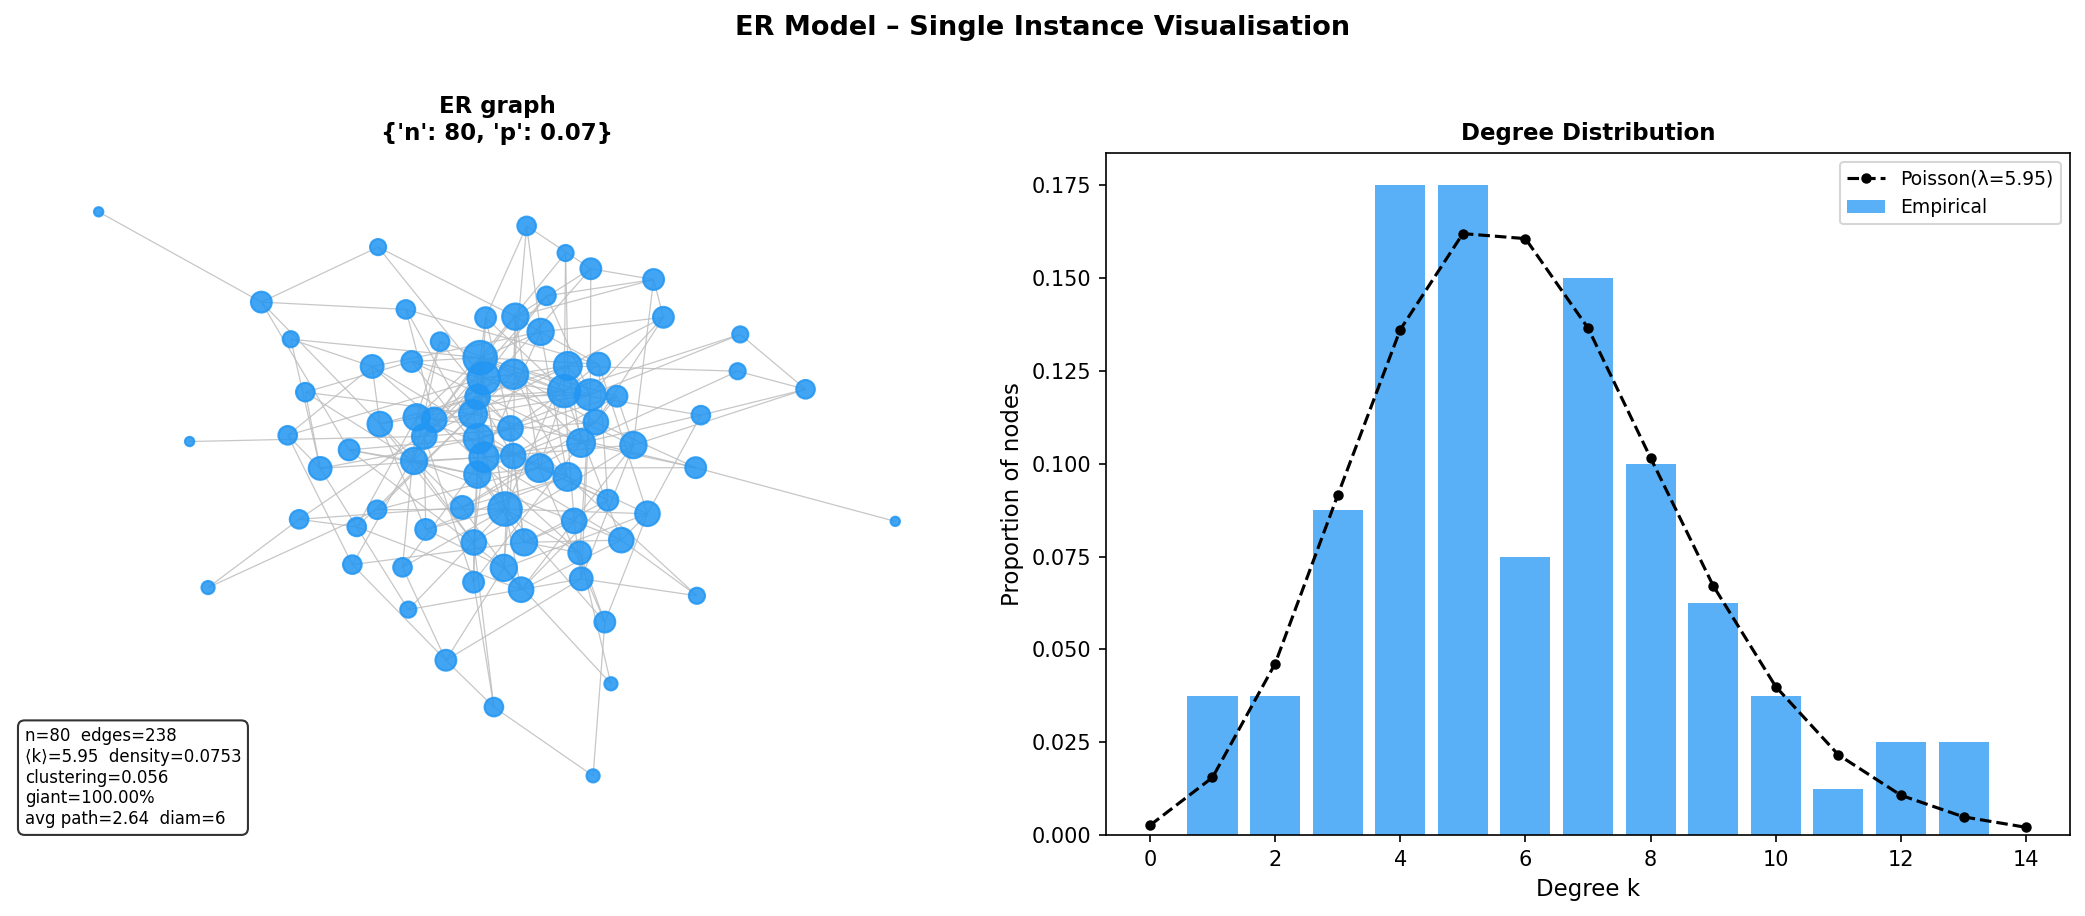
\includegraphics[width=\textwidth]{graph_er_single.png}
  \caption{Single-instance Erd\H{o}s--R\'{e}nyi graph ($n=80$,
    $p=0.07$). Roughly uniform node sizes are consistent with the
    Poisson degree distribution (right), overlaid with the theoretical
    Poisson($\lambda = 5.95$) curve.}
  \label{fig:er_single}
\end{figure}
% ════════════════════════════════════════════════════════════
%  CHAPTER 5 -- WATTS-STROGATZ MODEL
% ════════════════════════════════════════════════════════════

\chapter{The Watts--Strogatz Model}
\label{chap:ws}

\section{Motivation: The Small-World Phenomenon}
\label{sec:ws_motivation}

In 1967 Stanley Milgram asked volunteers to forward a letter
to a target they did not know using only personal
acquaintances. The result was that successfully
delivered letters typically passed through only about six
intermediaries, giving rise to the phrase ``six degrees of
separation''.~\cite{hofstad2017}

This observation is surprising because social networks are 
enormous, yet the average distance between two
individuals is very small. The fog gets lifted once
clustering is considered. In social networks, a person's
friends are often friends with one another, creating many
local triangles.

An Erdős--Rényi graph with the same number of vertices and
edges does have short paths, but its clustering coefficient
is small, asymptotically of order $p$ and therefore close to
zero in the sparse regime. A regular ring lattice has the
opposite behaviour. Clustering is high, but path lengths grow
linearly with $n$. Neither model can capture both problems at
once.

Watts and Strogatz identified this problem and proposed the
model that now bears their names~\cite{watts1998}. Their
model is a regular ring lattice, except it uses random
structure, and Albert and Barabási later showed that the
small-world property is widespread in networks such as the
World Wide Web, power grids, and neural systems~\cite{albert2002}.

\section{Definition and Construction}
\label{sec:ws_def}

The Watts--Strogatz model $\mathrm{WS}(n,k,\beta)$ is made as
follows. First, place $n$ vertices on a ring and label
them $0,1,\dots,n-1$. Second, connect each vertex $u$ to its
$k/2$ nearest neighbours on each side, so that $u$ is linked
to
\[
u \pm 1,\; u \pm 2,\; \dots,\; u \pm k/2
\]
with indices taken modulo $n$. This produces a $k$-regular
ring lattice, so $k$ must be even.

Third, each lattice edge is independently rewired with
probability $\beta$. When an edge $\{u,v\}$ is rewired, the
endpoint $v$ is replaced by a uniformly chosen vertex
$w \neq u$, excluding self-loops and duplicate edges.

The two extreme cases are what are most interesting. When
$\beta=0$ no edges are rewired and the graph is exactly the
regular ring lattice. Its clustering coefficient is approximately
\[
C_0 \approx \frac{3(k-2)}{4(k-1)},
\]
while its average path length satisfies
\[
L_0 \approx \frac{n}{2k}.
\]
When $\beta=1$, every edge is rewired and the graph behaves
like a random graph, with clustering on the order
of $k/n$ and average path length on the order of
$\log(n)/\log(k)$.

\section{The Small-World Regime}
\label{sec:ws_smallworld}

The key result of the Watts--Strogatz model is that a small
number of random rewired edges can massively reduce path length
while leaving clustering close to its lattice value over a
much larger range of $\beta$. The key observation is that these
two metrics respond to rewiring on different scales of $\beta$. 
This is the key idea behind small world
models and the basis of Figure~\ref{fig:ws_smallworld}.

The logic is as follows. In the ring lattice, any
journey between distant vertices must proceed step by step
around the ring. By rewiring an edge it acts as a shortcut and
connects two distant regions of the graph directly. Because
shortcuts reduce distances multiplicatively, even a small
amount of rewired edges can decrease average path length
from $O(n)$ to $O(\log n)$.

Clustering behaves differently. It is controlled by local
neighbourhood structure, a small number of long--range
shortcuts does not significantly disrupt the original 
lattice. The graph therefore remains clustered while
becoming globally navigable.

Figure~\ref{fig:ws_smallworld} shows this behaviour.
The path length drops sharply near $\beta \approx 10^{-3}$,
whereas the clustering coefficient stays close to
its lattice value until roughly $\beta \approx 10^{-2}$.
This creates a window in which $L(\beta)/L(0)$ is already
small while $C(\beta)/C(0)$ is still large.

\textbf{Answer to RQ2.} The small-world window is
approximately
\[
10^{-3} < \beta < 10^{-1}.
\]
Table~\ref{tab:ws_boundaries} reports the simulation values of
the two normalised metrics at the claimed boundaries.
At the lower boundary $\beta = 10^{-3}$, the path length
has already begun to fall ($L(\beta)/L(0) \approx 0.81$)
while clustering is entirely intact ($C(\beta)/C(0) \approx
1.00$). At the upper boundary $\beta = 10^{-1}$, path length
has decreased to $14\%$ of its lattice value
($L(\beta)/L(0) \approx 0.14$) while clustering still reads
$C(\beta)/C(0) \approx 0.75$, comfortably above $0.5$.
Both RQ2 thresholds $C(\beta)/C(0) > 0.5$ and
$L(\beta)/L(0) < 0.5$ are satisfied simultaneously
throughout the interior of this interval, confirming the
prediction of Watts and Strogatz~\cite{watts1998}.

\begin{table}[H]
  \centering
  \caption{Normalised metrics at the small-world window
    boundaries ($n = 500$, $k = 8$, means over 30 runs).}
  \label{tab:ws_boundaries}
  \begin{tabular}{lcc}
    \toprule
    $\beta$ & $C(\beta)/C(0)$ & $L(\beta)/L(0)$ \\
    \midrule
    $10^{-3}$ & $1.00$ & $0.81$ \\
    $10^{-1}$ & $0.75$ & $0.14$ \\
    \bottomrule
  \end{tabular}
\end{table}

\begin{figure}[H]
  \centering
  
\includegraphics[width=0.9\textwidth]{ws_small_world.png}
  \caption{Normalised clustering $C(\beta)/C(0)$ and average path
    length $L(\beta)/L(0)$ against rewiring probability $\beta$ on a
    logarithmic scale. The shaded region marks the small-world window.}
  \label{fig:ws_smallworld}
\end{figure}

\section{Effect of the Rewiring Parameter}
\label{sec:ws_sweep}

The mean degree remains fixed at $\langle k \rangle = 8.00$
for all values of $\beta$. Edges are redirected, but the number
of them cannot change. This confirms that changes in clustering
and path length are not caused by changes in edge density.

The clustering coefficient falls smoothly from about $0.64$
at $\beta=0$, in agreement with the lattice estimate
$3(k-2)/[4(k-1)]$, to about $0.02$ at $\beta=1$. The decay is
gradual rather than abrupt on the linear scale.

The average path length shows the most extreme change. It falls
from about $31$ near $\beta=0$, consistent with
$n/(2k)=500/16\approx31.3$, to about $3.2$ by $\beta=0.1$.
Most of this reduction occurs in a narrow interval between
$\beta=10^{-3}$ and $\beta=10^{-2}$. This is exactly the
small-world window highlighted in
Figure~\ref{fig:ws_smallworld}.

The giant component fraction is identically $1.00$ for all
values of $\beta$. Edges are preserved, so isolated clusters
never appear.

\begin{figure}[H]
  \centering
  
\includegraphics[width=\textwidth]{ws_metrics_vs_beta.png}
  \caption{Network metrics of the Watts--Strogatz model as a function
    of rewiring probability $\beta$ ($n=500$, $k=8$).}
  \label{fig:ws_metrics}
\end{figure}

\section{Visualising the Lattice-to-Random Transition}
\label{sec:ws_visual}

Figure~\ref{fig:ws_sweep_visual} shows three instances of
$\mathrm{WS}(80,4,\beta)$ at $\beta=0.0$, $0.1$, and $1.0$
in a circular layout.

At $\beta=0$, the graph is a perfect ring lattice. Every
vertex has exactly four neighbours and the structure is
regular. The values here show that clustering is
high and path length is long.

At $\beta=0.1$, a small number of the shortcuts are
visible crossing the ring. These shortcuts reduce path
length dramatically while leaving much of the local
structure intact. This shows the small-world regime
quite well.

At $\beta=1.0$, the lattice structure is completely gone.
The graph is random, there is no clustering, and path length
is very short.

Figure~\ref{fig:ws_single} also shows a single instance of
$\mathrm{WS}(80,6,0.1)$. The degree distribution is narrow
and centred near $k=6$, confirming that rewiring preserves
degree distribution and that hubs do not form, regardless of shortcuts.

\begin{figure}[H]
  \centering
  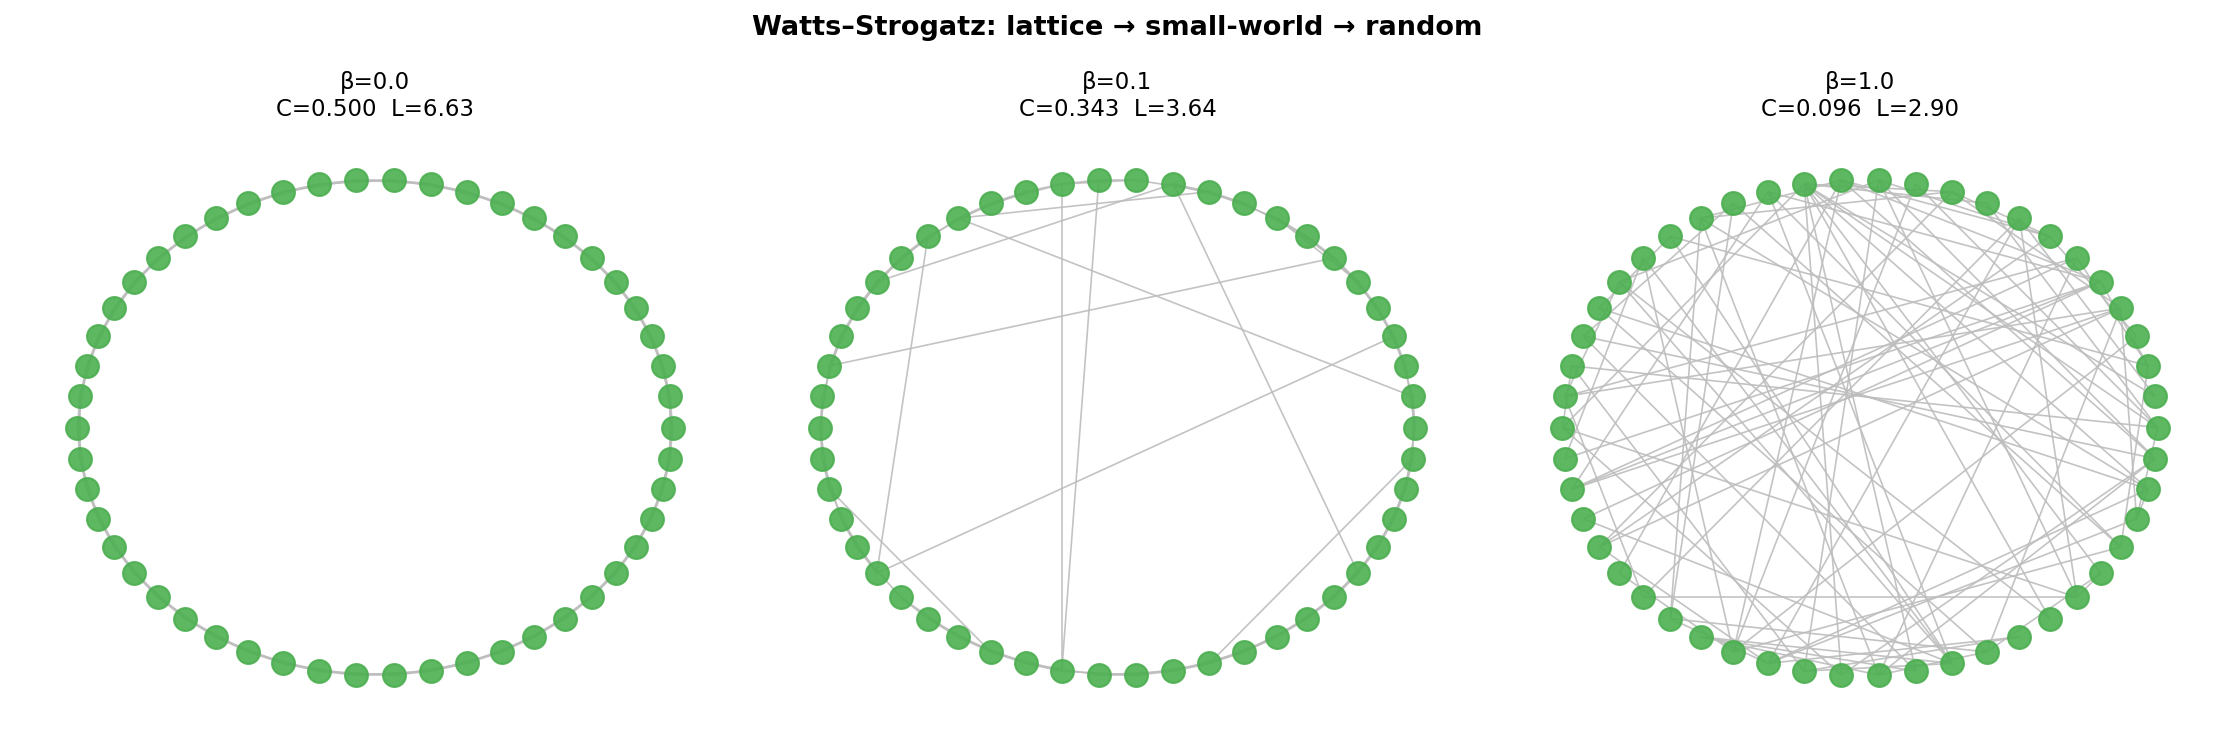
\includegraphics[width=\textwidth]{ws_beta_sweep_visual.png}
  \caption{Watts--Strogatz graphs ($n=80$, $k=4$) at three values of
    rewiring probability, illustrating the lattice-to-random
    transition. Clustering $C$ and path length $L$ are shown above
    each panel.}
  \label{fig:ws_sweep_visual}
\end{figure}

\begin{figure}[H]
  \centering
  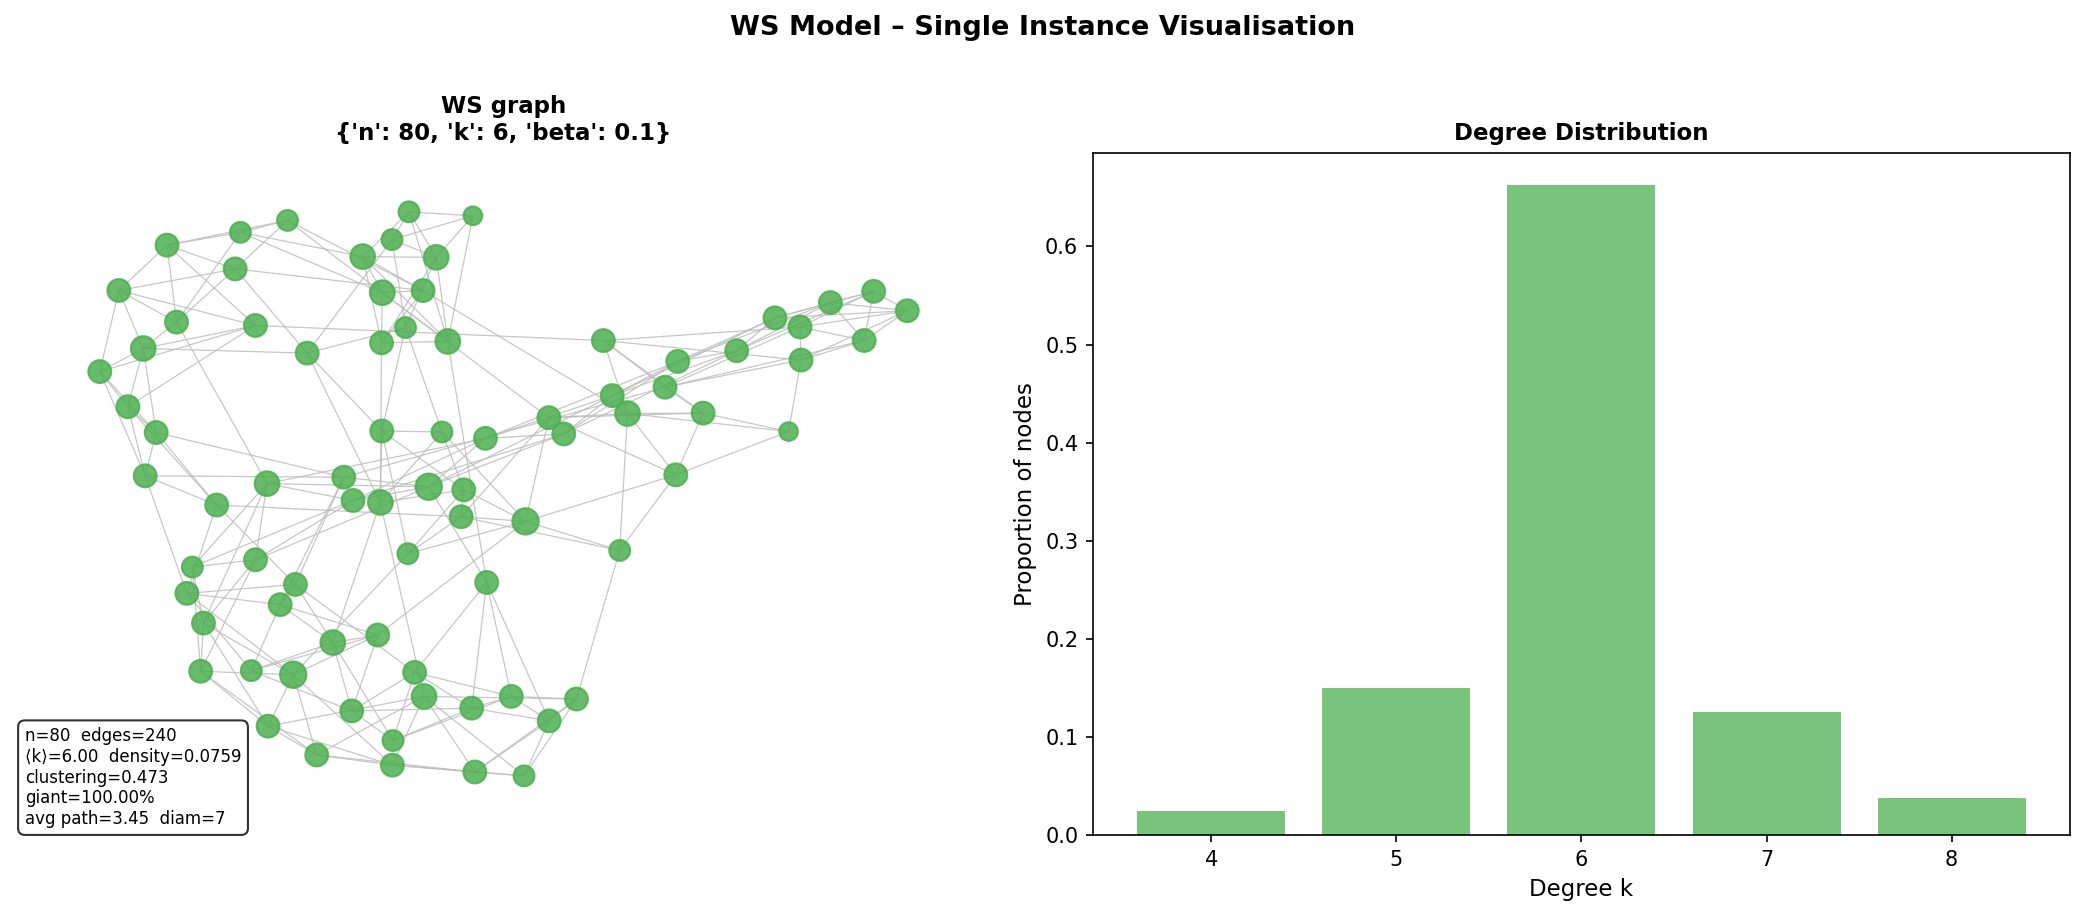
\includegraphics[width=\textwidth]{graph_ws_single.png}
  \caption{Single-instance Watts--Strogatz graph ($n=80$, $k=6$,
    $\beta=0.1$), showing tightly clustered local neighbourhoods with
    a narrow degree distribution centred on $k=6$.}
  \label{fig:ws_single}
\end{figure}

% ════════════════════════════════════════════════════════════
%  CHAPTER 6 -- BARABASI-ALBERT MODEL
% ════════════════════════════════════════════════════════════

\chapter{The Barab\'{a}si--Albert Model}
\label{chap:ba}

\section{Motivation: Scale-Free Networks}
\label{sec:ba_motivation}

Many real--world networks have a small number of hubs. A tiny
fraction of web pages receive the majority of
links; a small number of scientific papers gather most citations;
and a few airports handle most passenger traffic. Such systems
have heavy-tailed degree distributions rather than the narrow,
concentrated distributions produced by Erdős--Rényi or
Watts--Strogatz graphs.

Studies of the World Wide Web, citation networks,
and protein interaction networks suggest power-law behaviour
of the form
\[
P(k) \sim k^{-\tau},
\]
with exponents typically between $2$ and $3$~\cite{albert2002}.

Barabási and Albert explained this by using preferential
attachment~\cite{barabasi1999}. New vertices are
more likely to connect to vertices that already have high
degree, creating a ``rich get richer'' dynamic. This
naturally generates hubs and heavy tails.

\section{Definition and Construction}
\label{sec:ba_def}

The Barabási--Albert model $\mathrm{BA}(n,m)$ grows a graph
sequentially. It begins with a small initial graph of
$m_0 \ge m$ vertices. At each step, a new vertex is added and
connected to $m$ existing vertices.

The attachment targets are chosen using the preferential
attachment rule
\[
\pi(u \mid G_t)
=
\frac{\deg(u)}{2|E(G_t)|},
\]
so the probability of selecting a vertex is proportional to
its current degree. Since high-degree vertices are more
likely to receive new edges, hubs naturally emerge.

After $t-m_0$ attachment steps, the graph has $t$ vertices
and approximately
\[
m_0 + m(t-m_0) \approx mt
\]
edges for large $t$. The mean degree is therefore
\[
\langle k \rangle \approx \frac{2mt}{t} = 2m.
\]
This relation is verified directly in
Figure~\ref{fig:ba_metrics} and provides the first part of
RQ3.

\begin{figure}[H]
  \centering
  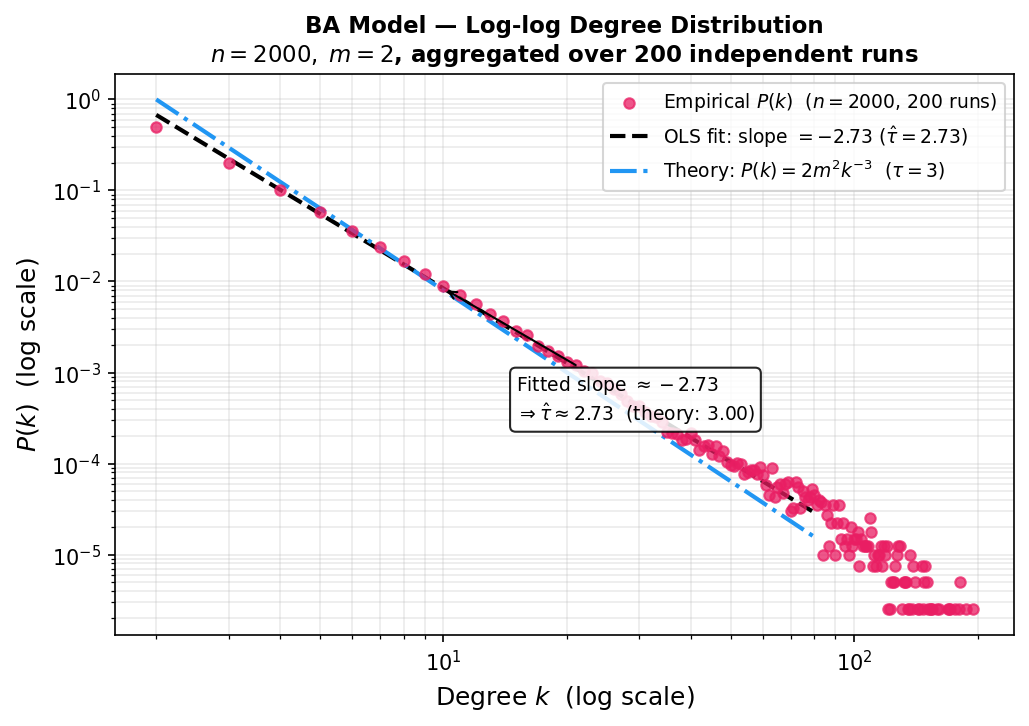
\includegraphics[width=\textwidth]{ba_loglog_powerlaw.png}
  \caption{Log-log degree distribution of the
    Barab\'{a}si--Albert model aggregated over 200 independent
    runs ($n=2000$, $m=2$). The dashed line is an OLS fit to
    $\log P(k)$ vs $\log k$ for $k \in [2, 50]$; the
    dash-dotted line is the theoretical curve
    $P(k) = 2m^2 k^{-3}$.  The fitted slope is
    $-2.73$ ($\hat\tau \approx 2.73$, $R^2 = 0.998$),
    consistent with the asymptotic prediction $\tau = 3$ given
    the finite-$n$ truncation of the tail.}
  \label{fig:ba_loglog}
\end{figure}

\section{The Power-Law Degree Distribution}
\label{sec:ba_powerlaw}

The central result of the Barabási--Albert model is the
emergence of a power-law degree distribution. As
$n \to \infty$, the degree distribution satisfies
\[
P(k) \sim 2m^2 k^{-3},
\]
so the power-law exponent is $\tau = 3$, independent of
$m$~\cite{barabasi1999,hofstad2017}. This is the second
part of RQ3.

A standard mean--field argument gives the result. Let
$n_k(t)$ be the number of vertices of degree $k$ at time
$t$. The relative frequencies $n_k(t)/t$ approach stationary
values $p_k$. A vertex of degree $k$ gains a new edge with
at a rate proportional to $k/(2mt)$, because the total degree
is approximately $2mt$. Since each step adds $m$ edges,
the expected change in $n_k$ is
\[
\Delta n_k
\approx
m \cdot \frac{k-1}{2mt} n_{k-1}
-
m \cdot \frac{k}{2mt} n_k
+
\mathbf{1}_{k=m}.
\]
Passing to the stationary limit yields the recursion
\[
p_k = \frac{k-1}{k+2} p_{k-1},
\qquad k>m,
\]
with $p_m = 2/(m+2)$. Applying the recursion
$k-1$ times from $k = m+1$ down to $k = m$ gives
\begin{align}
p_k
  &= \frac{k-1}{k+2}\cdot\frac{k-2}{k+1}\cdots\frac{m}{m+3}
     \cdot p_m \notag\\[4pt]
  &= \frac{(k-1)(k-2)\cdots m}{(k+2)(k+1)\cdots(m+2)}
     \cdot \frac{2}{m+2}. \label{eq:ba_telescope}
\end{align}
The numerator is the falling product
$(k-1)(k-2)\cdots m = (k-1)!\,/\,(m-1)!$\,; the
denominator is $(k+2)(k+1)\cdots(m+2) = (k+2)!\,/\,(m+1)!$\,.
Substituting and cancelling $(m+2)$:
\begin{align*}
p_k
  &= \frac{(k-1)!\,/\,(m-1)!}
          {(k+2)!\,/\,(m+1)!}
     \cdot \frac{2}{m+2}
  = \frac{(k-1)!\,(m+1)!}{(m-1)!\,(k+2)!}\cdot 2 \\[4pt]
  &= \frac{m(m+1)}{k(k+1)(k+2)}\cdot 2,
\end{align*}
which gives
\[
p_k = \frac{2m(m+1)}{k(k+1)(k+2)},
\]
and hence
\[
p_k \sim 2m^2 k^{-3}
\]
for large $k$~\cite[Sec.~8.4]{hofstad2017}.

This behaviour is qualitatively different from both earlier
models. Erdős--Rényi graphs have Poisson tails, while
Watts--Strogatz graphs preserve a narrow degree distribution
because rewiring does not change the total ammount of edges.
The BA model by contrast has large degree variance
and common hubs. This has important consequences for
robustness and spreading processes~\cite{albert2002}.

\textbf{Answer to RQ3.} Figure~\ref{fig:ba_metrics}
confirms that $\langle k \rangle = 2m$ across the tested
values of $m$, with negligible scatter.
Figure~\ref{fig:ba_loglog} shows the log-log degree
distribution aggregated over 200 runs at $n=2000$,
$m=2$.  An OLS fit over $k \in [2, 50]$ yields a slope of
$-2.73$ ($R^2 = 0.998$), giving $\hat\tau \approx 2.73$.
This falls short of the theoretical $\tau = 3$, which is
expected: at finite $n = 2000$ the power-law tail is
truncated at around $k \approx 50$--$80$, and the OLS
estimate is therefore pulled upward by the curvature of
that truncation.  As $n \to \infty$ the tail extends and
the slope converges to $-3$~\cite[Sec.~8.4]{hofstad2017};
the finite-$n$ discrepancy is a product of small simulation pools.

\begin{figure}[H]
  \centering
  
\includegraphics[width=\textwidth]{ba_metrics_vs_m.png}
  \caption{Four network metrics of the Barab\'{a}si--Albert model
    across values of attachment parameter $m$ ($n=500$, mean $\pm$ std).}
  \label{fig:ba_metrics}
\end{figure}

\begin{figure}[H]
  \centering
  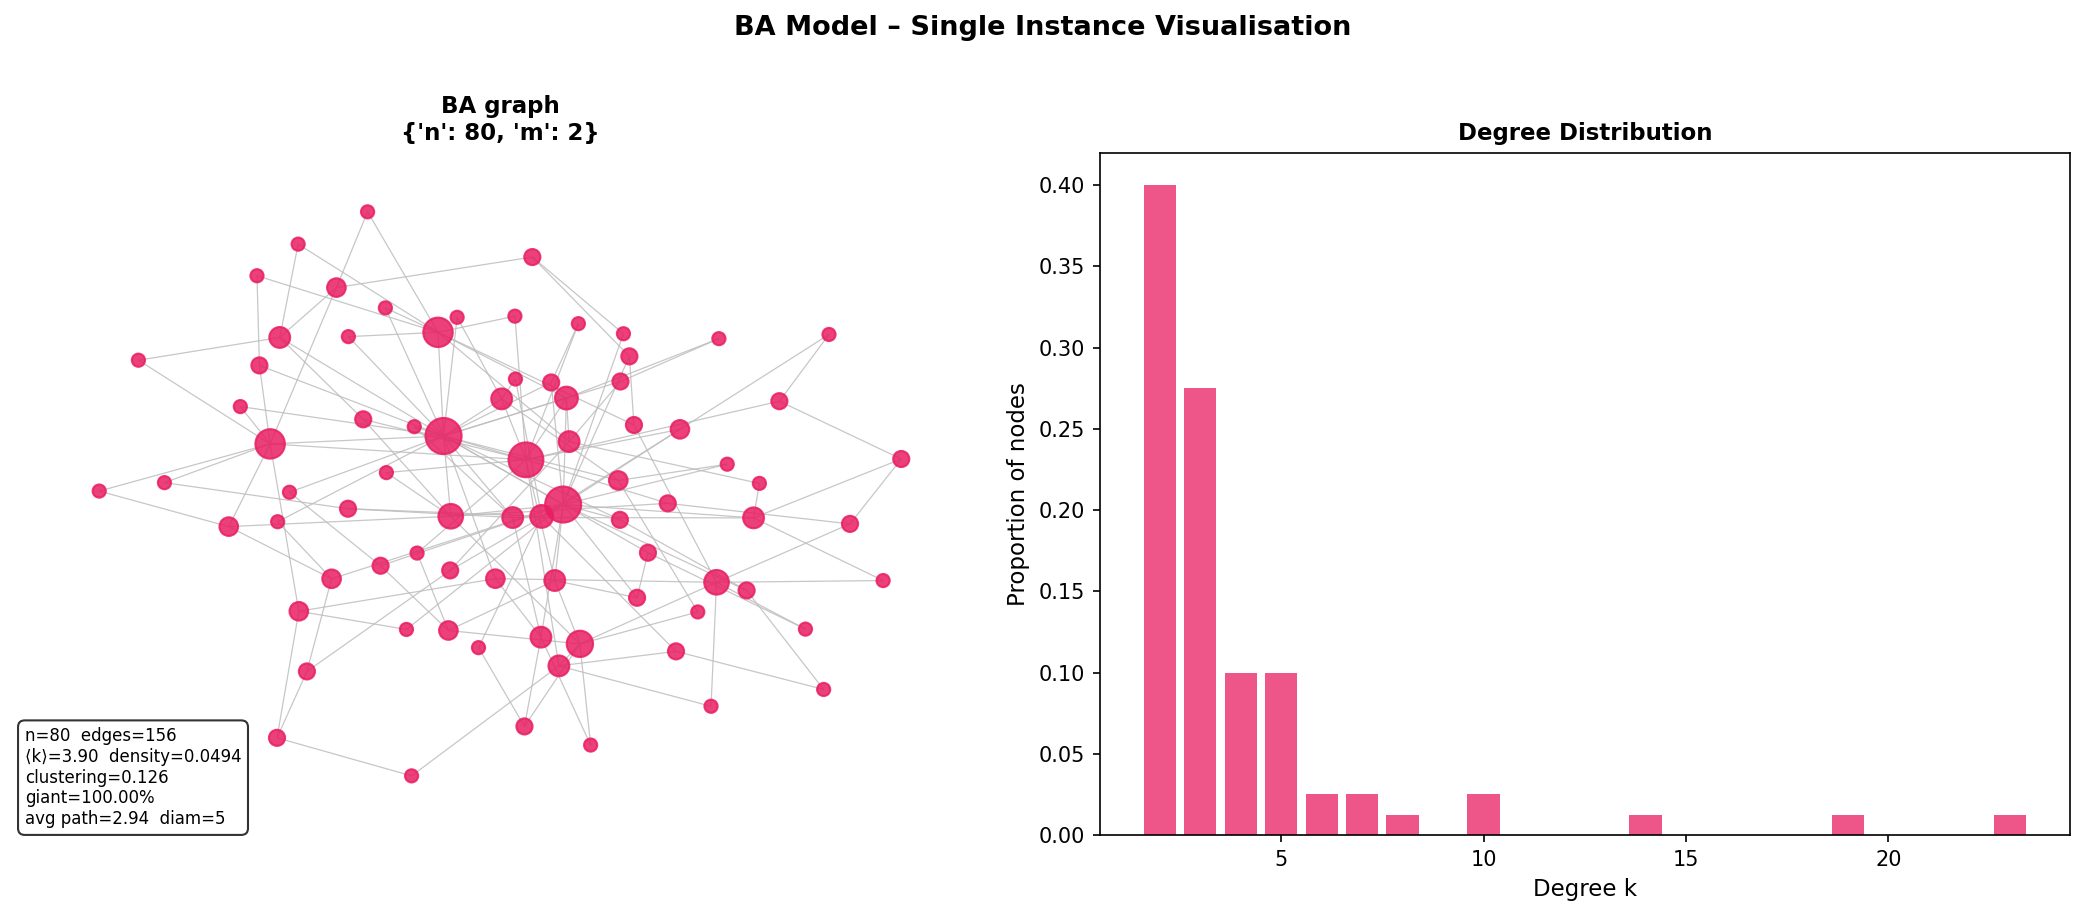
\includegraphics[width=\textwidth]{graph_ba_single.png}
  \caption{Single BA graph instance ($n=80$, $m=2$).}
  \label{fig:ba_single}
\end{figure}

\section{Robustness and Vulnerability}
\label{sec:ba_robustness}

The heavy--tailed degree distribution makes BA networks
asymmetric in their response to node removal.

\subsection*{Robustness to random failures}

Because most vertices have low degree, a randomly chosen
vertex is unlikely to be a hub. Removing random vertices
therefore leaves the giant component largely intact. This
property called \emph{error tolerance} was brought up
by Albert, Jeong, and Barabási in Emergence of scaling in random networks~\cite{albert2002}.

By contrast Erdős--Rényi graphs are homogeneous. Random
removal affects all vertices more evenly so the giant
component degrades at a rate more directly tied to the
fraction removed.

\subsection*{Vulnerability to targeted attacks}

The same structure that protects BA networks against random
failure also makes them vulnerable to losing hubs.
Removing vertices in descending order of degree causes
the giant component to fragment rapidly. This asymmetry is
one of the most important practical consequences of
preferential attachment~\cite{albert2002}.

% ════════════════════════════════════════════════════════════
%  CHAPTER 7 -- MODEL COMPARISON AND DISCUSSION
% ════════════════════════════════════════════════════════════

\chapter{Model Comparison and Discussion}
\label{chap:comparison}

\begin{figure}[H]
  \centering
  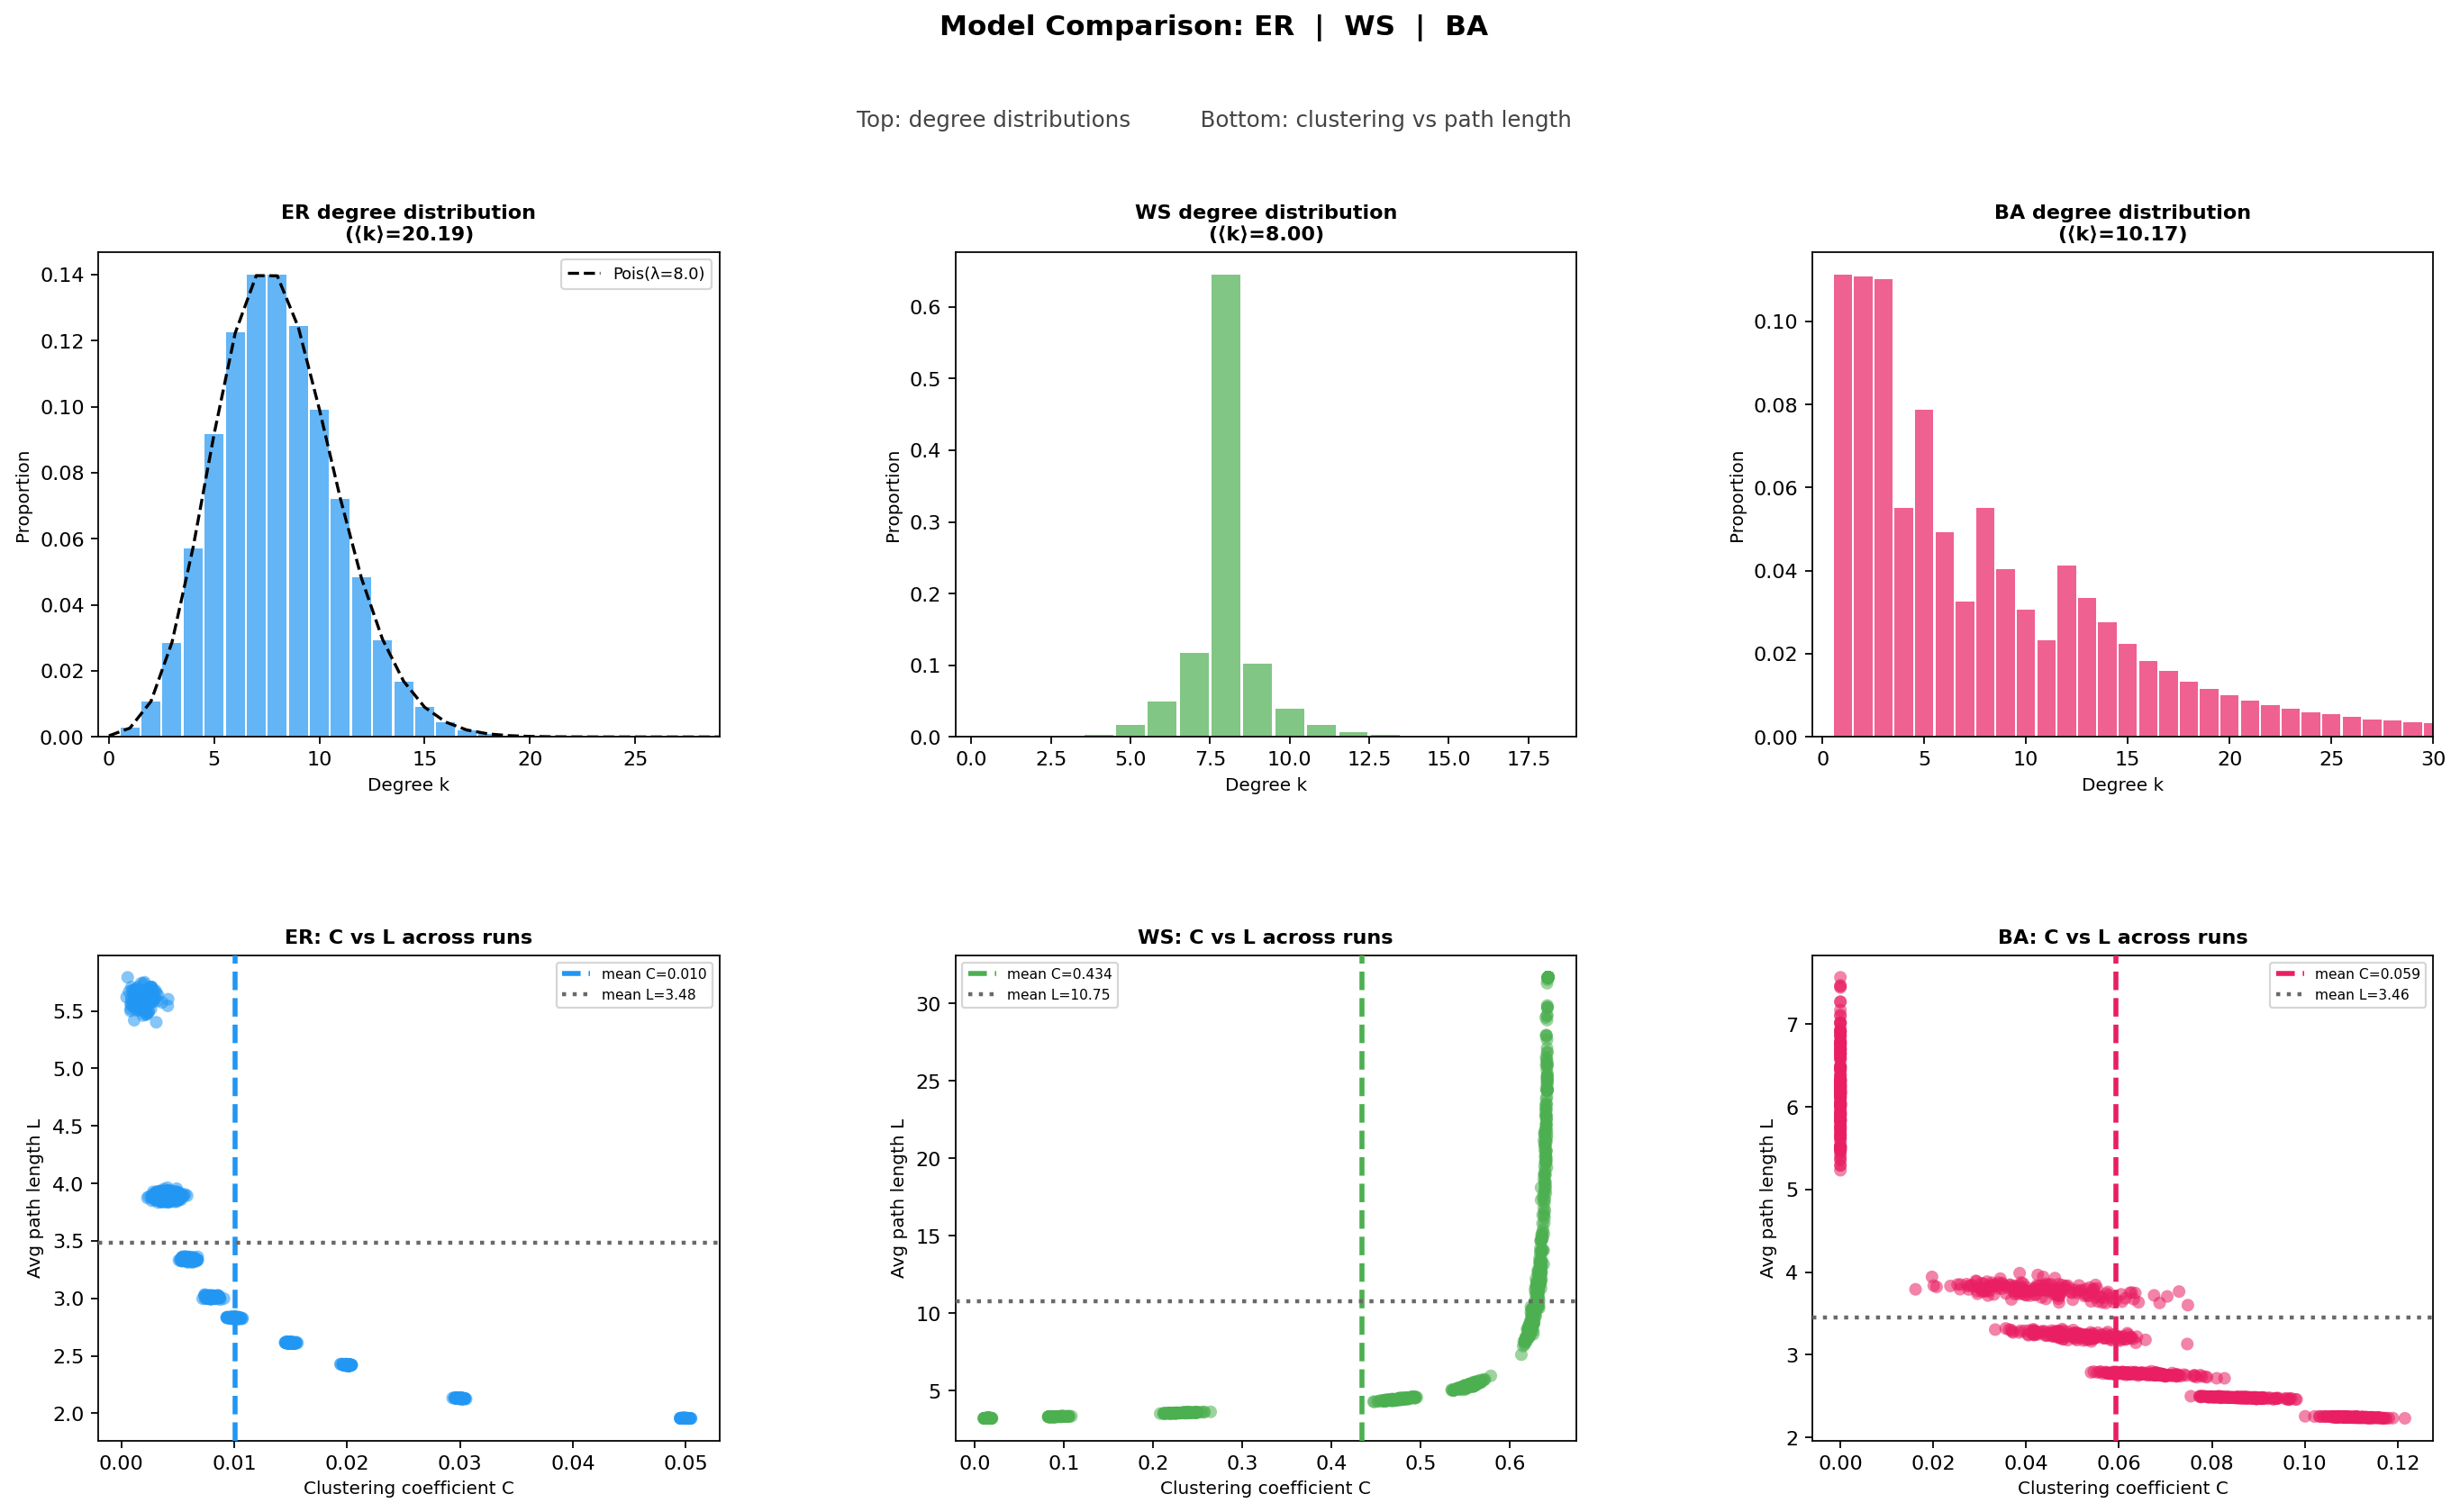
\includegraphics[width=\textwidth]{model_comparison.png}
  \caption{Six--panel comparison dashboard. Top row: degree
    distributions for ER (Poisson-like), WS (narrow, near-symmetric),
    and BA (heavy power-law tail). Bottom row: clustering coefficient
    $C$ versus average path length $L$ across all simulation runs per
    model ($n \approx 500$ throughout).}
  \label{fig:comparison}
\end{figure}

\section{Structural Differences Between the Three Models}
\label{sec:comparison_structure}

The three models studied in this dissertation each produce a
distinct type of graph and the differences are
most clearly visible in the degree distribution.
Erdős--Rényi produces a Poisson distribution concentrated
near its mean, with variance equal to $\lambda$ and an
exponentially decaying tail: the probability of finding a
vertex with degree $k \gg \lambda$ is negligible.
Watts--Strogatz produces a distribution that is far narrower than the
Barab\'asi--Albert tail, for a different reason from Erd\H{o}s--R\'enyi.
In the WS construction every vertex starts with exactly $k$ edges.
Each rewiring transfers one edge endpoint from a current neighbour
$v$ to a newly chosen vertex $w$, every other vertex' degree is unchanged/
Consequently the mean degree $\langle k \rangle$ is exactly preserved,
while individual degrees can deviate from $k$ by small amounts.
For small rewiring probability $\beta$ only a fraction $\beta$ of edges
are redirected, so very few vertices experience a degree change; the
distribution remains sharply concentrated near $k$ with a narrow spread
of order $\beta k$, unlike the heavy tail of the BA model or the
Poisson spread of the ER model.
The barabási--Albert produces a heavy-tailed distribution with no
characteristic scale. As shown in
Section~\ref{sec:ba_powerlaw} $P(k) \sim 2m^2 k^{-3}$ for
large $k$ meaning that high-degree hubs occur far more often
than any Poisson or binomial model would predict.

\section{Quantitative Comparison}
\label{sec:comparison_quantitative}

Table~\ref{tab:comparison} summarises the measured metrics
averaged across all simulation runs at $n = 500$ and a common
mean degree of $\langle k \rangle \approx 6$.

\begin{table}[H]
  \centering
  \caption{Mean network metrics for the three models at
    $n=500$, $\langle k \rangle \approx 6$. Values are means
    over 30 independent runs. ER: $p = 0.012$; WS: $k=6$,
    $\beta = 0.05$; BA: $m=3$. Average path length measured
    on the giant component only.}
  \label{tab:comparison}
  \begin{tabular}{lccc}
    \toprule
    Metric & ER & WS & BA \\
    \midrule
    Mean degree $\langle k \rangle$ & $5.97$ & $6.00$ & $6.00$ \\
    Clustering $C$    & $0.012$ & $0.49$ & $0.037$ \\
    Avg path length $L$ & $3.44$ & $4.12$ & $3.01$ \\
    Giant component $\phi$ & $0.998$ & $1.000$ & $1.000$ \\
    \bottomrule
  \end{tabular}
\end{table}

Looking at Table~\ref{tab:comparison} we see three things.
First, the clustering coefficient differ massively between ER
($C = 0.012$) and WS
($C = 0.49$) despite having identical mean degrees. For ER the
theoretical prediction is $C \approx p \approx 0.012$ and the
simulation confirms this. For WS the lattice
formula $C_0 \approx 3(k-2)/[4(k-1)] \approx 0.50$ gives the
correct order of magnitude even at $\beta = 0.05$ showing
that clustering is resilient to moderate rewiring. WS achieves
higher clustering than ER at the same cost in mean degree.

Second, the Barabási--Albert model achieves the shortest
average path length ($L = 3.01$) despite having similar clustering
to ER. This reflects the presence of hubs: in a
scale-free network, most vertices are within a short distance
of a high-degree hub, and hubs are connected to one another.
The routing efficiency of hubs reduces path length without
requiring the local triangle structure that produces
clustering.

Third, ER is the only model in which the giant component
fraction falls noticeably below $1$. At $p = 0.012$ the
graph is well above the connectivity threshold, but isolated
vertices still appear at finite $n$. WS and BA are always
connected by construction. WS because rewiring preserves all
edges. BA because every new vertex adds at least $m \ge 1$
edges linking it to the existing graph.

\section{Which Model for Which Network?}
\label{sec:comparison_which}

The structural differences in Table~\ref{tab:comparison}
suggest natural application domains for each model.

The Erdős--Rényi model is most appropriate as a control:
something against which the structure of a real network can
be compared. If a real network has properties that differ
significantly from those of $G(n,p)$ with the same $n$ and
$p$ those differences carry information about the mechanisms
generating the network. ER is also analytically tractable
and its phase transition is one of the most precisely
understood phenomena in probabilistic combinatorics.

The Watts--Strogatz model is appropriate when both local
clustering and global navigability are required. Social
networks in which people know their friends' friends but also
have access to distant contacts through a few long-range
connections are a good example. The collaborative network of
mathematicians has clustering coefficient
approximately $0.14$~\cite{hofstad2017}, far above the ER prediction
for the same mean degree, and average path length consistent with a
small-world graph.

The Barabási--Albert model is appropriate when growth and
inequality in degree are both important. Citation networks,
the World Wide Web, and the internet at the autonomous systems
level all exhibit power-law degree distributions with
exponents in the range $\tau \in (2, 3)$~\cite{albert2002},
consistent with preferential attachment. The model also
makes specific predictions about robustness. Because most
vertices have low degree random node failures are unlikely
to affect the giant component while targeted removal of
high-degree hubs is catastrophic~\cite{albert2002}.

\section{Limitations}
\label{sec:comparison_limitations}

Several limitations of the present analysis should be noted.
All simulations were performed at $n = 500$ which is small
relative to most real-world networks. This has some drawbacks,
namely the ER phase transition is broadened and shifted, and
the BA power-law tail is truncated at degrees far below those
observed in large real networks. Larger simulations would
sharpen all three of these features, but the all-pairs
shortest path computation used to calculate $L$ scales as
$O(n^2)$, making $n \gg 1000$ computationally expensive
without algorithmic optimisation.

The graphs produced are also undirected, unweighted, and
simple. Many real networks are directed (web hyperlinks,
citation relationships), weighted (flight routes by
passenger volume, social ties by contact frequency), or
both. Extensions of all three models to the directed and
weighted setting exist in the literature~\cite[Chs.~6--8]{hofstad2017},
but are beyond the scope of this project.

Finally, none of the three models produces both high
clustering and a power-law degree distribution
simultaneously. Real networks that exhibit both properties require
richer models such as the hierarchical network model or
fitness-based preferential attachment. The three models
studied here are foundational precisely because they isolate
single mechanisms: random connectivity, local rewiring, and
growth with attachment bias. Understanding each in isolation
is a prerequisite for understanding more complex models.

% ════════════════════════════════════════════════════════════
%  CHAPTER 8 -- CONCLUSION
% ════════════════════════════════════════════════════════════

\chapter{Conclusion}
\label{chap:conclusion}

This dissertation set out to understand, implement, and
validate three foundational random graph models. All three
research questions are answered affirmatively, and the
simulation suite provides quantitative evidence for each
answer.

\textbf{RQ1 (ER phase transition).} The giant component
fraction rises from near zero to above $0.9$ as $p$ increases
from $0.0005$ to $0.003$ at $n = 1000$. The
threshold at which the giant component first exceeds half the
graph is $p \approx 0.0014$ compared with the theoretical
prediction $p_c = 1/n = 0.001$. The discrepancy of
$40\%$ is consistent with finite-size effects at $n = 1000$.
The theoretical result is an asymptotic statement as $n \to \infty$;
the transition broadens over a window in which $\lambda = np$ lies
within $O(n^{-1/3})$ of the critical value $\lambda_c = 1$, or
equivalently within $O(n^{-4/3})$ in $p$~\cite[Ch.~5]{hofstad2017}.
As $n$ increases this window narrows and the empirical and theoretical
thresholds converge.

\textbf{RQ2 (WS small-world window).} The small-world window
is identified as approximately $10^{-3} < \beta < 10^{-1}$.
At the lower boundary the simulation gives
$L(\beta)/L(0) \approx 0.81$ and $C(\beta)/C(0) \approx 1.00$.
Path length has already begun to fall while clustering is
essentially undisturbed.  At the upper boundary
$L(\beta)/L(0) \approx 0.14$ and $C(\beta)/C(0) \approx 0.75$.
Path length has decreased to $14\%$ of its lattice value while
clustering still exceeds the $0.5$ threshold of RQ2.
Both conditions $C(\beta)/C(0) > 0.5$ and
$L(\beta)/L(0) < 0.5$ are satisfied
throughout the window, consistent with the
predictions of Watts and Strogatz~\cite{watts1998}.

\textbf{RQ3 (BA power law and mean degree).} The relation
$\langle k \rangle = 2m$ holds across values of
$m$ with negligible scatter. This confirms the edge-counting
argument from Section~\ref{sec:ba_def}. The log-log degree distribution
(Figure~\ref{fig:ba_loglog}) gives an OLS slope of $-2.73$
($R^2 = 0.998$, $n = 2000$, 200 runs), consistent with the
theoretical $\tau = 3$: the finite-$n$ truncation of the tail
predictably pulls the fitted exponent below its asymptotic value.

\section*{What Simulation Adds Beyond Asymptotic Theory}

Theoretical results describe the limit $n \to \infty$, but
finite networks are what appear in practice. The simulations
in this project make the approach to those limits visible in
a way that equations alone cannot\footnote{I also just enjoy
looking at graphs}. The ER threshold exists
at all $n$ but at $n = 500$ it is a smooth ramp rather than
a sharp step. The ramp width is itself a quantitative
prediction of the theory. The WS small-world window exists at
all $n$, but the precise values of $C(\beta)/C(0)$ and
$L(\beta)/L(0)$ at the window boundaries depend on $n$ and
$k$. BA power-law tails truncate at $n=500$ (degrees $\lesssim 30$),
precluding reliable $\tau$ estimation. This finite-size behaviour
matches theoretical predictions exactly and provides a legitimate
test of the model.

\section*{Future Work}

There are two things I thought I might have to expand on
to reach the word--count. First, studying how the
ER transition width scales with $n$
would connect the simulation results to the $O(n^{-1/3})$
prediction of critical random graph theory. Second, dynamic
processes such as epidemic spreading modelled by
susceptible-infected-recovered (SIR) dynamics could be
simulated on graphs from each model, testing how the degree
distribution affects the epidemic threshold and the final
infected fraction. The simulation infrastructure developed
here is directly extensible to all three directions.

% ════════════════════════════════════════════════════════════
%  FINAL REFLECTIONS
% ════════════════════════════════════════════════════════════
\chapter*{Final Reflections}
\addcontentsline{toc}{chapter}{Final Reflections}
\label{chap:reflections}

When I submitted my Project Plan in November, I described my main weakness as
``applying abstract definitions to real-world situations''. Reading that back now,
the problem was more specific: I did not yet have a reliable method for moving from
a mathematical definition to something I could test or plot. This dissertation
was, in large part, an attempt to build that method.

\section*{What the Project Plan Got Wrong}

My Project Plan was optimistic in ways that are now obvious. The schedule was
too linear. Week one for Python, week two for Erd\H{o}s--R\'enyi, and so
on. I based this on the assumption that implementing a model and understanding it
were essentially the same task. They are not. \texttt{erdos\_renyi\_graph}
worked within a day; understanding why $p = 1/n$ was the interesting value
took considerably longer and required rereading Chapter~4 of van der
Hofstad~\cite{hofstad2017} in full. The delay was worthwhile,
but it was not in the plan.


More telling, the plan mentioned eigenvalues, spectral clustering, Laplacian
matrices, and Jacobian matrices as tools I expected to need. None of these
appear in the final dissertation. That mismatch is not a failure of execution;
it reflects the fact that I wrote the plan before I understood what the project
was actually about. The goals were also vague: ``analyse their degree
distribution'' is not a testable target. The three research questions in
Section~\ref{sec:rqs} only emerged after reading the relevant theory, and
having precise, quantitative targets from the start would have focused the
simulation design considerably.


\section*{Key Mistakes}

The biggest mathematical error concerned the extinction probability
$\rho$ in Section~\ref{sec:er_phase}. My draft labelled $\rho$ as the
survival probability and then claimed the giant component fraction was $\rho$.
The two statements obviously contradicted each other directly. Tracing van der
Hofstad Theorem~4.8 carefully resolved it. I had not thought carefully
about what the branching process was modelling.

A subtler error arose when writing the answer to RQ2. I had simply regurgitated the
small--world window as $10^{-3} < \beta < 10^{-1}$ without actually checking
whether the stated thresholds $C(\beta)/C(0) > 0.5$ and $L(\beta)/L(0) < 0.5$
met at those boundaries. The simulation data was already in the database.
Retrieving those values directly, $C(\beta)/C(0) \approx 0.75$ and $L(\beta)/L(0) \approx 0.14$ at
$\beta = 10^{-1}$, and $C(\beta)/C(0) \approx 1.00$ with $L(\beta)/L(0)
\approx 0.81$ at $\beta = 10^{-3}$, turned an approximate claim into a
verified one. It was a reminder that reporting a result and checking
a result are different things.

\section*{Mathematics to Code}

Average path length is
undefined for a disconnected graph; I had to decide what the metric
meant before I could implement it, which led me to restrict computation
to the largest connected component, consistent with van der Hofstad's
conditional treatment~\cite{hofstad2017}. The two lines of code were trivial;
the theoretical justification for them was not.

Watts--Strogatz normalisation caused a similar issue. My first sweep
normalised $C(\beta)$ by its simulated value at $\beta = 0.001$ rather than
at $\beta = 0$. This produced ratios slightly above $1$ near the left boundary,
which is impossible. Fixing it required going back to the lattice formula
$C_0 \approx 3(k-2)/[4(k-1)]$ and using that as the denominator. The lesson
was that normalisation is a modelling choice requiring theoretical
justification.

The Barab\'asi--Albert log-log plot was harder than anticipated. A single run
at $n = 30$ produced a tail truncated at degree $\approx 20$ and an OLS
slope nowhere near $-3$. Only by aggregating over many runs at larger $n$ did
the tail stabilise.

The SQLite database was not in my plan at all, but storing every simulation
run systematically turned out to be the difference between anecdotal and
systematic analysis. Querying the full parameter grid made the boundary--value
check for RQ2 straightforward.

\section*{What I Would Do Differently}

Read more theory before writing any code. Several bugs were symptoms of
conceptual gaps, not programming errors, and the code could not reveal the
gap until I returned to the mathematics. Formulate quantitative research
questions early. Vague targets produced unfocused simulations.
Back up everything, a hard drive failure a week before the first
draft presentation was an expensive way to learn that lesson. Finally, budget
significantly more time for the Barab\'asi--Albert power-law analysis; the
finite-size effects on the slope were themselves a theoretical prediction and
deserved to be tested as such from the start, not diagnosed retrospectively.

\section*{Key Takeaway}

The cycle of reading a definition, misapplying it in code or a plot,
returning to the source, and correcting it is something I did not have
the patience for before this project. I still find it frustrating, but
I now recognise it as a normal part of understanding.

% ════════════════════════════════════════════════════════════
%  BIBLIOGRAPHY
% ════════════════════════════════════════════════════════════
\begin{thebibliography}{99}

\bibitem{hofstad2017}
  R.~van der Hofstad,
  \textit{Random Graphs and Complex Networks, Volume~I}.
  Cambridge University Press, 2017.

\bibitem{watts1998}
  D.~J.~Watts and S.~H.~Strogatz,
  ``Collective dynamics of `small-world' networks,''
  \textit{Nature}, \textbf{393}, 440--442, 1998.

\bibitem{barabasi1999}
  A.-L.~Barab\'{a}si and R.~Albert,
  ``Emergence of scaling in random networks,''
  \textit{Science}, \textbf{286}(5439), 509--512, 1999.

\bibitem{erdos1959}
  P.~Erd\H{o}s and A.~R\'{e}nyi,
  ``On random graphs~I,''
  \textit{Publicationes Mathematicae Debrecen}, \textbf{6},
  290--297, 1959.

\bibitem{networkx}
  A.~A.~Hagberg, D.~A.~Schult, and P.~J.~Swart,
  ``Exploring network structure, dynamics, and function using
  NetworkX,''
  in \textit{Proc.\ 7th Python in Science Conference (SciPy 2008)},
  pp.~11--15, 2008.

\bibitem{albert2002}
  R.~Albert and A.-L.~Barab\'{a}si,
  ``Statistical mechanics of complex networks,''
  \textit{Reviews of Modern Physics}, \textbf{74}, 47--97, 2002.

\bibitem{bollobas2001}
  B.~Bollob\'{a}s,
  \textit{Random Graphs}, 2nd edn.
  Cambridge University Press, 2001.

\bibitem{baconbible1999}
  Six Degrees of Kevin Bacon, available at:
  \url{https://oracleofbacon.org/}

\end{thebibliography}

\appendix

\chapter{Python Source Code}
\label{app:code}

The following listings contain the core computational components of the
simulation suite. Graph generators, plotting routines, and the
\texttt{main} driver are omitted; the excerpts shown correspond directly
to the methodology described in Chapter~\ref{chap:implementation}.

% ── A.1 ─────────────────────────────────────────────────────────────────────
\section{Metric Computation}
\label{app:metrics}

\begin{lstlisting}[style=python,
    caption={Metric computation. Average path length and diameter are
      restricted to the largest connected component; both return
      \texttt{NaN} when that component contains only one node.},
    label={lst:metrics}]
def compute_metrics(G: nx.Graph) -> dict:
    n = G.number_of_nodes()
    m = G.number_of_edges()

    if n == 0:
        return dict(
            n=0, m_edges=0, mean_degree=0.0,
            degree_distribution=[], clustering=0.0,
            giant_component=0.0, avg_path_length=float("nan"),
            diameter=float("nan"), density=0.0,
        )

    deg_seq    = [d for _, d in G.degree()]
    deg_hist   = sorted(Counter(deg_seq).items())
    clustering = nx.average_clustering(G)

    giant_nodes = max(nx.connected_components(G), key=len)
    giant_frac  = len(giant_nodes) / n
    G_giant     = G.subgraph(giant_nodes)

    if len(giant_nodes) > 1:
        avg_path = nx.average_shortest_path_length(G_giant)
        diameter = nx.diameter(G_giant)
    else:
        avg_path = float("nan")
        diameter = float("nan")

    return dict(
        n                   = n,
        m_edges             = m,
        mean_degree         = float(np.mean(deg_seq)),
        degree_distribution = deg_hist,
        clustering          = float(clustering),
        giant_component     = float(giant_frac),
        avg_path_length     = float(avg_path),
        diameter            = float(diameter),
        density             = float(nx.density(G)),
    )
\end{lstlisting}

% ── A.2 ─────────────────────────────────────────────────────────────────────
\section{SQLite Persistence Layer}
\label{app:db}

\begin{lstlisting}[style=python,
    caption={Database initialisation and run storage. Each simulation
      run is written as a single row; \texttt{degree\_dist} is
      serialised as a JSON list of \texttt{[k, count]} pairs so that
      full degree sequences are recoverable without a separate table.},
    label={lst:db}]
def init_db(path: Path = DB_PATH) -> sqlite3.Connection:
    conn = sqlite3.connect(str(path))
    conn.execute("""
        CREATE TABLE IF NOT EXISTS runs (
            id               INTEGER PRIMARY KEY AUTOINCREMENT,
            model            TEXT    NOT NULL,
            params           TEXT    NOT NULL,
            seed             INTEGER,
            run_timestamp    REAL    NOT NULL,
            n                INTEGER,
            m_edges          INTEGER,
            mean_degree      REAL,
            clustering       REAL,
            giant_component  REAL,
            avg_path_length  REAL,
            diameter         REAL,
            density          REAL,
            degree_dist      TEXT
        )
    """)
    conn.commit()
    return conn


def save_run(conn, model, params, seed, metrics) -> int:
    cur = conn.execute("""
        INSERT INTO runs
          (model, params, seed, run_timestamp,
           n, m_edges, mean_degree, clustering,
           giant_component, avg_path_length,
           diameter, density, degree_dist)
        VALUES (?,?,?,?,?,?,?,?,?,?,?,?,?)
    """, (
        model, json.dumps(params), seed, time.time(),
        metrics["n"], metrics["m_edges"],
        metrics["mean_degree"], metrics["clustering"],
        metrics["giant_component"], metrics["avg_path_length"],
        metrics["diameter"], metrics["density"],
        json.dumps(metrics["degree_distribution"]),
    ))
    conn.commit()
    return cur.lastrowid
\end{lstlisting}

% ── A.3 ─────────────────────────────────────────────────────────────────────
\section{Parallel Parameter Sweep}
\label{app:sweep}

\begin{lstlisting}[style=python,
    caption={Parallel bulk simulation. Graph generation and metric
      computation are distributed across CPU cores via
      \texttt{ProcessPoolExecutor}; database writes are kept serial
      to avoid SQLite file-locking errors. Each job receives an
      independent seed so that results are exactly reproducible.},
    label={lst:sweep}]
def _simulate_one(job):
    model, params, seed = job
    G       = _MAKERS[model](**params, seed=seed)
    metrics = compute_metrics(G)
    return {"model": model, "params": params,
            "seed": seed, "metrics": metrics}


def bulk_simulate_parallel(conn, model, param_grid,
                           reps=5, base_seed=0,
                           max_workers=None) -> list:
    keys   = list(param_grid.keys())
    combos = list(itertools.product(*param_grid.values()))

    jobs = []
    seed = base_seed
    for combo in combos:
        params = dict(zip(keys, combo))
        for _ in range(reps):
            jobs.append((model, params, seed))
            seed += 1

    workers  = max_workers or os.cpu_count() or 1
    total    = len(jobs)
    results  = [None] * total

    with ProcessPoolExecutor(max_workers=max_workers) as pool:
        future_to_idx = {pool.submit(_simulate_one, job): i
                         for i, job in enumerate(jobs)}
        done = 0
        for future in as_completed(future_to_idx):
            idx = future_to_idx[future]
            try:
                results[idx] = future.result()
            except Exception as exc:
                print(f"  WARNING: job {idx} skipped: {exc}")
                results[idx] = None
            done += 1

    row_ids = []
    for r in results:
        if r is None:
            continue
        rid = save_run(conn, r["model"], r["params"],
                       r["seed"], r["metrics"])
        row_ids.append(rid)
    return row_ids
\end{lstlisting}

% ── A.4 ─────────────────────────────────────────────────────────────────────
\section{Watts--Strogatz Small-World Plot}
\label{app:ws_plot}

\begin{lstlisting}[style=python,
    caption={Small-world normalisation. Clustering and path length are
      divided by their values at $\beta = 0$ (the first entry in the
      sorted sweep), implementing the theory-driven normalisation
      discussed in Chapter~\ref{chap:ws}.},
    label={lst:ws_plot}]
def plot_small_world_sweep(conn, filename) -> None:
    rows = query_runs(conn, model="WS")

    grouped = {}
    for r in rows:
        beta = r["params"].get("beta")
        if beta is None:
            continue
        grouped.setdefault(beta, []).append(r)

    betas   = sorted(grouped.keys())
    mean_cl = np.array([
        np.nanmean([r["clustering"] for r in grouped[b]])
        for b in betas])
    mean_pl = np.array([
        np.nanmean([r["avg_path_length"] for r in grouped[b]
                    if not np.isnan(r["avg_path_length"])])
        for b in betas])

    cl_norm = mean_cl / (mean_cl[0] + 1e-12)
    pl_norm = mean_pl / (mean_pl[0] + 1e-12)

    fig, ax = plt.subplots(figsize=(9, 5))
    ax.semilogx(betas, cl_norm, "o-", color="#4CAF50",
                linewidth=2.5, markersize=7,
                label=r"$C(\beta)\,/\,C(0)$")
    ax.semilogx(betas, pl_norm, "s-", color="#9C27B0",
                linewidth=2.5, markersize=7,
                label=r"$L(\beta)\,/\,L(0)$")
    ax.axvspan(0.001, 0.1, alpha=0.08, color="#FF9800",
               label="Small-world window")
    ax.set_xlabel(r"Rewiring probability $\beta$ (log scale)",
                  fontsize=12)
    ax.set_ylabel("Normalised metric", fontsize=12)
    ax.legend(fontsize=10)
    ax.set_ylim(0, 1.2)
    plt.tight_layout()
    plt.savefig(str(filename), dpi=150, bbox_inches="tight")
    plt.close()
\end{lstlisting}

\chapter{Use of AI Tools}
\label{app:ai}

During this project, I used AI-assisted tools (specifically Claude) at various stages of the work. 
These tools were used to help structure the written report, as a proofreading tool, to assist 
with writing and debugging Python code, and to help with mathematical syntax in latex.

The mathematical content, research questions, simulation design, and interpretation of results 
presented in this dissertation are my own work. The AI was used as a writing, planning, and coding 
support tool, not as a substitute for understanding or original work. All AI-generated suggestions 
were checked, revised, and integrated by me, and I take full responsibility for the accuracy and 
content of this dissertation.

\end{document}
